\documentclass{article}
\usepackage[utf8]{inputenc}
\usepackage{indentfirst}
\usepackage{tikz}
\usepackage[paper=portrait,pagesize]{typearea}
\usepackage{tabularx}
\usepackage{bchart}
\usepackage{eso-pic}
\usepackage{xcolor}
\usepackage[margin=4cm]{geometry}
\usepackage[hidelinks]{hyperref}
\usepackage[toc,page]{appendix}
\usetikzlibrary{shapes,calc}

%% Define Boxes of Elements  
\newcommand{\CommonElementTextFormat}[4]
{
  \begin{minipage}{2.2cm}
    \centering
      {\textbf{#1} \hfill #2}%
      \linebreak \linebreak
      {\textbf{#3}}%
      \linebreak \linebreak
      {{#4}}
  \end{minipage}
}

\newcommand{\NaturalElementTextFormat}[4]
{
  \CommonElementTextFormat{#1}{#2}{\LARGE {#3}}{#4}
}


%% Define 'footlabel'
\newcommand{\footlabel}[2]{%
    \addtocounter{footnote}{1}%
    \footnotetext[\thefootnote]{%
        \addtocounter{footnote}{-1}%
        \refstepcounter{footnote}\label{#1}%
        #2%
    }%
    $^{\ref{#1}}$%
}

\newcommand{\footref}[1]{%
    $^{\ref{#1}}$%
}

%% Fill Color Styles
\tikzstyle{AlkaliMetalFill} = [fill=blue!55]
\tikzstyle{AlkalineEarthMetalFill} = [fill=blue!40]
\tikzstyle{TransitionMetalFill} = [fill=blue!25]
\tikzstyle{PostTransitionMetalFill} = [fill=orange!25]
\tikzstyle{MetalloidFill} = [fill=yellow!15]
\tikzstyle{NonmetalFill} = [fill=green!25]
\tikzstyle{HalogenFill} = [fill=green!40]
\tikzstyle{NobleGasFill} = [fill=green!55]
\tikzstyle{LanthanideFill} = [fill=purple!50]
\tikzstyle{ActinideFill} = [fill=purple!25]
\tikzstyle{UnknownFill} = [fill=gray!25]

%% Element Styles
\tikzstyle{AlkaliMetal} = [draw=black, AlkaliMetalFill, minimum width=2.75cm, minimum height=2.75cm, node distance=2.75cm]
\tikzstyle{AlkalineEarthMetal} = [AlkaliMetal, AlkalineEarthMetalFill]
\tikzstyle{TransitionMetal} = [AlkaliMetal, TransitionMetalFill]
\tikzstyle{PostTransitionMetal} = [AlkaliMetal, PostTransitionMetalFill]
\tikzstyle{Metalloid} = [AlkaliMetal, MetalloidFill]
\tikzstyle{Nonmetal} = [AlkaliMetal, NonmetalFill]
\tikzstyle{Halogen} = [AlkaliMetal, HalogenFill]
\tikzstyle{NobleGas} = [AlkaliMetal, NobleGasFill]
\tikzstyle{Lanthanide} = [AlkaliMetal, LanthanideFill]
\tikzstyle{Actinide} = [AlkaliMetal, ActinideFill]
\tikzstyle{Unknown} = [AlkaliMetal, UnknownFill]
\tikzstyle{PeriodLabel} = [font={\sffamily\LARGE}, node distance=2.0cm]
\tikzstyle{GroupLabel} = [font={\sffamily\LARGE}, minimum width=2.75cm, node distance=2.0cm]
\tikzstyle{TitleLabel} = [font={\sffamily\Huge\bfseries}]

%% Center Boxes According to Text
\newbox\mybox
\def\centerfigure#1{%
  \setbox\mybox\hbox{#1}%
  \raisebox{-0.43\dimexpr\ht\mybox+\dp\mybox}{\copy\mybox}%
}

\begin{document}

\lineskip = 0.25cm

%% Cover Page
\begingroup
\thispagestyle{empty}
\AddToShipoutPicture*{\put(0,0){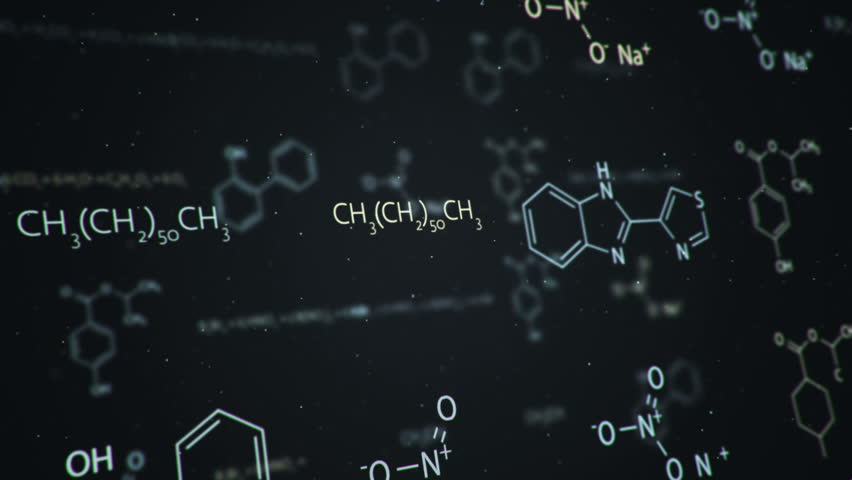
\includegraphics[scale=1.76]{./resources/Front}}}
\centering {
    \vspace*{-0.01cm}
    \Huge\sffamily\selectfont\textcolor{white}{\textbf{Chemical Elements}}\par
    \vspace*{0.5cm}
    
    \LARGE\textcolor{white}{Obtaining chemical elements that constitute everyday words}\par
    \vspace*{8.6cm}
}

\hfill
\begin{minipage}{0.3\textwidth}
    \centering\LARGE\sffamily\selectfont {
        \textcolor{white}{João Barreira}
        
        \vspace{0.3cm}
        
        \textcolor{white}{Mafalda Nunes}
    }\par
\end{minipage}

\vspace{5.2cm}


{\Large\par\sffamily\selectfont\hfill \textcolor{white}{Scripting e Processamento de Linguagem Natural}}

\endgroup
\newpage

%% Obtained Text
\section{Obtained Text}

\textbf{What Are Elements and Compounds?}



\textit{Abstract}

The definitions of elements and compounds have changed very little in the past 200 years, but chemistry itself has changed a great deal over time. Any form of an element has been considered as the element itself and a compound had to have an exact atomic composition that included two or more different elements. This commentary suggests that only the atomic form of each element should be considered as the element and most other forms should be called elementary substances. A publication of the International Union of Pure and Applied Chemistry (IUPAC) has stated that compounds can be formed by a single element. The author agrees that in terms of modern chemical bonding both heteronuclear and homonuclear molecules can be considered as compounds.



\textit{Article}

This question was brought to my attention by an article(1) in this Journal entitled: “A2: Element or Compound?” This article shows the result of quizzes given to students and the correct response according to the authors is that the gas A2 is an element. \scalebox{0.3}{
  \centerfigure{\begin{tikzpicture}[font=\sffamily, transform shape]
    \node[name=I, Nonmetal, rounded corners=.15cm, node distance=3cm] {\hyperlink{subsubsection::I}{\NaturalElementTextFormat{53}{126.904}{I}{Iodine}}};
  \end{tikzpicture}}
} was disturbed by this, but \scalebox{0.3}{
  \centerfigure{\begin{tikzpicture}[font=\sffamily, transform shape]
    \node[name=I, Nonmetal, rounded corners=.15cm, node distance=3cm] {\hyperlink{subsubsection::I}{\NaturalElementTextFormat{53}{126.904}{I}{Iodine}}};
  \end{tikzpicture}}
} find that this concept of elements and compounds is given in most introductory chemistry courses. \scalebox{0.3}{
  \centerfigure{\begin{tikzpicture}[font=\sffamily, transform shape]
    \node[name=In, PostTransitionMetal, rounded corners=.15cm, node distance=3cm] {\hyperlink{subsubsection::In}{\NaturalElementTextFormat{49}{114.818}{In}{Indium}}};
  \end{tikzpicture}}
} a common textbook,(2) these definitions are found in the glossary under element: “(1) A substance which cannot be separated into simpler components by using chemical techniques. (2) A substance consisting of atoms of the same atomic number. Examples: hydrogen; gold; uranium.” Also in the same textbook a compound is described as “...an electrically neutral substance that consists of two or more different elements with their atoms present in a definite ratio.” Versions similar to this can be found in most of the textbooks that \scalebox{0.3}{
  \centerfigure{\begin{tikzpicture}[font=\sffamily, transform shape]
    \node[name=I, Nonmetal, rounded corners=.15cm, node distance=3cm] {\hyperlink{subsubsection::I}{\NaturalElementTextFormat{53}{126.904}{I}{Iodine}}};
  \end{tikzpicture}}
} could find. It seems that these definitions have been in use for over 150 years. The first definition under elements is commonly attributed to Lavoisier. Surely our definition of chemical techniques has changed a great deal since then. The purpose of this commentary is to initiate a reconsideration as to how, in the 21st century, should we define elements and compounds?

Two recent Nobel Prizes have been given for the preparation of substances that this definition would simply call elements. A Chemistry Prize was given for the isolation of the interesting molecule C60\footlabel{C60}{This formula has the IUPAC name \textbf{(C{60}-I{h})[5,6]fullerene} and the molecular formula \textbf{C60}. Some alternative names are Fullerene, Fullerene C60, Buckminsterfullerene and 99685-96-8. Its complexity has value 2030. The exact mass is 720. The molecular weight is 720.66. The monoisotopic mass is 720. }, and the most recent Physics Prize was given for obtaining graphene from graphite. Both these new forms of carbon have chemical bonding that gives them very interesting physical and chemical properties. Should we dismiss them as simply elements or even allotropes? \scalebox{0.3}{
  \centerfigure{\begin{tikzpicture}[font=\sffamily, transform shape]
    \node[name=In, PostTransitionMetal, rounded corners=.15cm, node distance=3cm] {\hyperlink{subsubsection::In}{\NaturalElementTextFormat{49}{114.818}{In}{Indium}}};
  \end{tikzpicture}}
} the case of oxygen, we also have the very important molecule, ozone. It is formed in the upper atmosphere and it protects all living things from the harmful effects of ultraviolet light from the sun. Ozone is a triatomic molecule with a well-defined molecular structure, it has an electric dipole moment, and it is closely related to both sulfur dioxide and disulfur monoxide.

The concept of an element is very old and \scalebox{0.3}{
  \centerfigure{\begin{tikzpicture}[font=\sffamily, transform shape]
    \node[name=F, Nonmetal, rounded corners=.15cm, node distance=3cm] {\hyperlink{subsubsection::F}{\NaturalElementTextFormat{9}{18.998}{F}{Fluorine}}};
  \end{tikzpicture}}
}. A. Paneth’s article(3) entitled, “The Epistemological Status of the Chemical Concept of Element”, traces it back to Aristotle. Our thinking is very physical and is based on modern physics and astronomy. Data in these fields tell us that all the matter on our earth was generated by complicated and violent nuclear events that created our atomic nuclei. These nuclei are the components of ordinary matter and they form the chemical elements. The first list of chemical elements came from classical analytical chemistry. The periodic table introduced systematics for these elements, and every textbook gives this table a prominent place. Our understanding of the nature of the elements shown in the periodic table has changed over the years. Analytical chemists knew nothing of atoms, nuclei, and electrons, and so any form of each element was taken as the element itself. One hundred years ago, we discovered that each chemical element possesses a nucleus that had a unique positive charge and is surrounded by electrons, which fill most of the volume of the element. Soon we learned about the s, p, d, and f orbitals and about the energies of the electrons in these orbitals. With this understanding, the reasons for the strange periodicity of the periodic table became clear. It was then seen that each chemical element was a unique atom and the common forms of the elements are the result of these atoms bonding together.

We have now learned how to generate and study atoms, and the atoms in the periodic table can be directly used to do chemistry. We can ask what form of each element are we listing in this table? For the symbol in the periodic table “\scalebox{0.3}{
  \centerfigure{\begin{tikzpicture}[font=\sffamily, transform shape]
    \node[name=C, Nonmetal, rounded corners=.15cm, node distance=3cm] {\hyperlink{subsubsection::C}{\NaturalElementTextFormat{6}{12.011}{C}{Carbon}}};
  \end{tikzpicture}}
}”, do we mean graphite, diamond, or even C60\footref{C60}? The chemistry of each of these forms is different, but the position in the table is established by the charge on the nucleus of the atom and the bonding properties of its electrons. \scalebox{0.3}{
  \centerfigure{\begin{tikzpicture}[font=\sffamily, transform shape]
    \node[name=As, Metalloid, rounded corners=.15cm, node distance=3cm] {\hyperlink{subsubsection::As}{\NaturalElementTextFormat{33}{74.922}{As}{Arsenic}}};
  \end{tikzpicture}}
} a result, the symbol “\scalebox{0.3}{
  \centerfigure{\begin{tikzpicture}[font=\sffamily, transform shape]
    \node[name=C, Nonmetal, rounded corners=.15cm, node distance=3cm] {\hyperlink{subsubsection::C}{\NaturalElementTextFormat{6}{12.011}{C}{Carbon}}};
  \end{tikzpicture}}
}” in the periodic table means the atom and not its various forms. So we should reserve the designation element to the atom that possess electrons in s, p, d, and f orbitals that determine its chemistry. \scalebox{0.3}{
  \centerfigure{\begin{tikzpicture}[font=\sffamily, transform shape]
    \node[name=In, PostTransitionMetal, rounded corners=.15cm, node distance=3cm] {\hyperlink{subsubsection::In}{\NaturalElementTextFormat{49}{114.818}{In}{Indium}}};
  \end{tikzpicture}}
} Linus Pauling’s College Chemistry,(4) he stated: “The kind of matter represented by a particular kind of atom is called an element.” This is followed by: “All pure substances can be divided into two classes: elementary substances and compounds.” J. E. Early’s recent article(5) goes over many of the historical aspects of elements and substances mentioned by Paneth,(3) but he does take the position that H2\footlabel{H2}{This formula has the IUPAC name \textbf{molecular hydrogen} and the molecular formula \textbf{H2}. Some alternative names are Hydrogen, Dihydrogen, Molecular hydrogen and 1333-74-0. The exact mass is 2.016. The molecular weight is 2.016. The monoisotopic mass is 2.016. } and O2\footlabel{O2}{This formula has the IUPAC name \textbf{molecular oxygen} and the molecular formula \textbf{O2}. Some alternative names are Oxygen, Molecular oxygen, oxygen molecule and Dioxygen. The exact mass is 31.99. The molecular weight is 31.998. The monoisotopic mass is 31.99. } should be called an “elementary substance” and not the element itself.

\scalebox{0.3}{
  \centerfigure{\begin{tikzpicture}[font=\sffamily, transform shape]
    \node[name=In, PostTransitionMetal, rounded corners=.15cm, node distance=3cm] {\hyperlink{subsubsection::In}{\NaturalElementTextFormat{49}{114.818}{In}{Indium}}};
  \end{tikzpicture}}
} the older textbooks, one can find the historical basis for the definition of compounds. Early chemistry was based entirely on chemical analysis. \scalebox{0.3}{
  \centerfigure{\begin{tikzpicture}[font=\sffamily, transform shape]
    \node[name=In, PostTransitionMetal, rounded corners=.15cm, node distance=3cm] {\hyperlink{subsubsection::In}{\NaturalElementTextFormat{49}{114.818}{In}{Indium}}};
  \end{tikzpicture}}
} this analysis, once one had reached the point of identifying the amounts and number of elements present in a sample, the analysis ceased, for that is as far as simple chemical analysis could go. Compounds were identified if they satisfied the laws of definite proportions, multiple proportions, and equivalent proportions, even when most of the compounds examined at that time were not very pure.(6) \scalebox{0.3}{
  \centerfigure{\begin{tikzpicture}[font=\sffamily, transform shape]
    \node[name=In, PostTransitionMetal, rounded corners=.15cm, node distance=3cm] {\hyperlink{subsubsection::In}{\NaturalElementTextFormat{49}{114.818}{In}{Indium}}};
  \end{tikzpicture}}
} 1860, as part of the finalization of the atomic weight scale, it was decided that the common elemental gases, which were known at that time, were all diatomic molecules. They were still called elements and not compounds, despite being diatomic, for that is what chemical analysis concluded. \scalebox{0.3}{
  \centerfigure{\begin{tikzpicture}[font=\sffamily, transform shape]
    \node[name=In, PostTransitionMetal, rounded corners=.15cm, node distance=3cm] {\hyperlink{subsubsection::In}{\NaturalElementTextFormat{49}{114.818}{In}{Indium}}};
  \end{tikzpicture}}
} the 20th century we developed X-ray crystallography, molecular spectroscopy, and quantum mechanical methods to determine molecular structure, and we can even calculate the properties of chemical bonds. We learned that the difference between diamond and graphite is the nature of their chemical bonds. Discussion of chemical bonding has become an important part of chemistry. For example, when we discuss chemical bonding, molecular nitrogen, N2\footlabel{N2}{This formula has the IUPAC name \textbf{molecular nitrogen} and the molecular formula \textbf{N2}. Some alternative names are Nitrogen, Nitrogen gas, Molecular nitrogen and 7727-37-9. Its complexity has value 8. The exact mass is 28.006. The molecular weight is 28.014. The monoisotopic mass is 28.006. }, is our example of a triple bond. We also compare it to the isoelectronic “chemical compound”, \scalebox{0.3}{
  \centerfigure{\begin{tikzpicture}[font=\sffamily, transform shape]
    \node[name=C, Nonmetal, rounded corners=.15cm, node distance=3cm] {\hyperlink{subsubsection::C}{\NaturalElementTextFormat{6}{12.011}{C}{Carbon}}};
  \end{tikzpicture}}
}
+
\scalebox{0.3}{
  \centerfigure{\begin{tikzpicture}[font=\sffamily, transform shape]
    \node[name=O, Nonmetal, rounded corners=.15cm, node distance=3cm] {\hyperlink{subsubsection::O}{\NaturalElementTextFormat{8}{15.999}{O}{Oxygen}}};
  \end{tikzpicture}}
}. The chemical bonds in these two molecules are very closely related, and from the viewpoint of chemical bonds, molecular nitrogen is as much of a compound as is \scalebox{0.3}{
  \centerfigure{\begin{tikzpicture}[font=\sffamily, transform shape]
    \node[name=C, Nonmetal, rounded corners=.15cm, node distance=3cm] {\hyperlink{subsubsection::C}{\NaturalElementTextFormat{6}{12.011}{C}{Carbon}}};
  \end{tikzpicture}}
}
+
\scalebox{0.3}{
  \centerfigure{\begin{tikzpicture}[font=\sffamily, transform shape]
    \node[name=O, Nonmetal, rounded corners=.15cm, node distance=3cm] {\hyperlink{subsubsection::O}{\NaturalElementTextFormat{8}{15.999}{O}{Oxygen}}};
  \end{tikzpicture}}
}. The gases in our atmosphere are commonly called oxygen and nitrogen, but their modern names(7) are dioxygen and dinitrogen.

One can try to look past current textbooks for a more modern definition of a compound, and a colleague suggested the publications of the International Union of Pure and Applied Chemistry (IUPAC). The authors make recommendations in their publications for all sorts of chemical matters. If one looks in the IUPAC booklet,(8) “Principles of Chemical Nomenclature”, there is first a discussion of the elements in the periodic table and their symbols. Next is a discussion of substances and compounds. A key statement in this discussion is: “Compounds are composed of atoms of the same or more than one kind of element in some form of chemical combination.” A little later they also state: “An elementary substance is a physical form of that element, as it may be prepared and studied.”

The IUPAC definition of compounds is very broad, and it also seems to take issue with the concept that a compound has to have an exact whole number chemical formula. The modern high temperature \scalebox{0.3}{
  \centerfigure{\begin{tikzpicture}[font=\sffamily, transform shape]
    \node[name=Y, TransitionMetal, rounded corners=.15cm, node distance=3cm] {\hyperlink{subsubsection::Y}{\NaturalElementTextFormat{39}{88.906}{Y}{Yttrium}}};
  \end{tikzpicture}}
}
+
\scalebox{0.3}{
  \centerfigure{\begin{tikzpicture}[font=\sffamily, transform shape]
    \node[name=B, Metalloid, rounded corners=.15cm, node distance=3cm] {\hyperlink{subsubsection::B}{\NaturalElementTextFormat{5}{10.81}{B}{Boron}}};
  \end{tikzpicture}}
}
+
\scalebox{0.3}{
  \centerfigure{\begin{tikzpicture}[font=\sffamily, transform shape]
    \node[name=C, Nonmetal, rounded corners=.15cm, node distance=3cm] {\hyperlink{subsubsection::C}{\NaturalElementTextFormat{6}{12.011}{C}{Carbon}}};
  \end{tikzpicture}}
}
+
\scalebox{0.3}{
  \centerfigure{\begin{tikzpicture}[font=\sffamily, transform shape]
    \node[name=O, Nonmetal, rounded corners=.15cm, node distance=3cm] {\hyperlink{subsubsection::O}{\NaturalElementTextFormat{8}{15.999}{O}{Oxygen}}};
  \end{tikzpicture}}
} super conductors have formulas such as YBa2Cu3O7–x. An x value of 0.15 gives the highest superconductive temperature. X-ray scattering shows that \scalebox{0.3}{
  \centerfigure{\begin{tikzpicture}[font=\sffamily, transform shape]
    \node[name=Y, TransitionMetal, rounded corners=.15cm, node distance=3cm] {\hyperlink{subsubsection::Y}{\NaturalElementTextFormat{39}{88.906}{Y}{Yttrium}}};
  \end{tikzpicture}}
}
+
\scalebox{0.3}{
  \centerfigure{\begin{tikzpicture}[font=\sffamily, transform shape]
    \node[name=B, Metalloid, rounded corners=.15cm, node distance=3cm] {\hyperlink{subsubsection::B}{\NaturalElementTextFormat{5}{10.81}{B}{Boron}}};
  \end{tikzpicture}}
}
+
\scalebox{0.3}{
  \centerfigure{\begin{tikzpicture}[font=\sffamily, transform shape]
    \node[name=C, Nonmetal, rounded corners=.15cm, node distance=3cm] {\hyperlink{subsubsection::C}{\NaturalElementTextFormat{6}{12.011}{C}{Carbon}}};
  \end{tikzpicture}}
}
+
\scalebox{0.3}{
  \centerfigure{\begin{tikzpicture}[font=\sffamily, transform shape]
    \node[name=O, Nonmetal, rounded corners=.15cm, node distance=3cm] {\hyperlink{subsubsection::O}{\NaturalElementTextFormat{8}{15.999}{O}{Oxygen}}};
  \end{tikzpicture}}
} has a well-defined localized order and a less well-defined long-range order. Although it may not satisfy the classical definition of a compound, it is clearly a compound that has been altered or doped to improve certain properties.

It is clear that chemistry teachers should stay away from exam questions about elements and compounds for the correct answers are uncertain, but what should we now suggest to textbook authors? The first message is that it is time to consider the old definitions as purely historical. Chemistry has gotten very complex over the last 50 years and the textbook authors have to simplify, but the classical definitions of elements and compounds are too out-of-date for what we now know about chemistry. Above all, the designation of element should be reserved for the atoms themselves, and for the common forms of the elements, the designation of elementary substances should be used. For the designation as compounds it is not clear what most authors will do. One approach is just to forget the historical definition and follow the approach given by IUPAC, but for some teachers schooled in the old ways that might be too much. We know that all molecules are unique, held together by the same kinds of chemical bonds regardless of whether the nuclei are identical or not. \scalebox{0.3}{
  \centerfigure{\begin{tikzpicture}[font=\sffamily, transform shape]
    \node[name=As, Metalloid, rounded corners=.15cm, node distance=3cm] {\hyperlink{subsubsection::As}{\NaturalElementTextFormat{33}{74.922}{As}{Arsenic}}};
  \end{tikzpicture}}
} a compromise, we offer the following designations: chemical substances and elementary substances. Chemical substances are compounds if they have formula weights that are not simply atomic weights. It seems logical that all molecules should be called compounds. This would mean that dinitrogen, ozone, and C60\footref{C60}, which have their unique formula weights, could be called compounds, but metallic gold or graphite, which have no unique formula weight, should be called elementary substances. \scalebox{0.3}{
  \centerfigure{\begin{tikzpicture}[font=\sffamily, transform shape]
    \node[name=At, Metalloid, rounded corners=.15cm, node distance=3cm] {\hyperlink{subsubsection::At}{\NaturalElementTextFormat{85}{210.0}{At}{Astatine}}};
  \end{tikzpicture}}
} the same time, some authors might be more radical and say that all substances held together by chemical bonds are compounds. We could even invent the term elementary compound, but that would seem to be unnecessary. We should also give up the idea that chemistry is devoted entirely to making pure compounds. Many of the most important substances these days are prepared not to be pure and can be called materials or doped compounds.





\textbf{Chemical Elements}



\textit{Their Classfication}



THE recognition of certain properties, the association of certain ideals with the several elements, is a necessary step in classifying the elements in accordance with MendeleJeff's great generalization—or rather it may be said to be both involved in and an outcome of Mendelejeff's conception. Until recently our difficulty was to understand the relationship of the metallic and the non-metallic elements; now we are confronted with another problem — that of the existence of inert “paraffinoid” elements. 

It is commonly assumed that these are monatomic, but the evidence on which this assumption is based is absolutely unconvincing, and would be generally admitted to be so were we in the habit of looking before we leapt to conclusions. Assuming that the elements are compounds, the formation of inert compounds does not appear to be out of place, in view of the existence of practically inert hydrocarbons. But, on the other hand, in view of the properties of nitrogen, which is one of the most active of substances in the monatomic state, although an inert gas in the diatomic condition, it may well be that the inertness of helium and the other a member of the argon group is also simulated. 

Sir James Dewar's; observations have shown that helium and charcoal have no inconsiderable affinity at the toiling point of the former, which is within five • degrees of the absolute zero, the molecular heat of absorption (apart from that due to liquefaction) of helium at that temperature being apparently as high as about sixty calories. The proof he has also given that helium alone does not convey an electric discharge is also of significance since the pas- Rage of a discharge through it under ordinary conditions is an indication that it can be included with ether substances in a conducting system. Such evidence as there is therefore points to the elements under discussion being different from the others only in the degree of stability of their molecules. 

Of late years the difficulty of classifying the elements has been increased rather than diminished, not merely because of the discovery of the inert gases but also on account of the apparent impossibility of ordering the position of an element such as tellurium in accordance with its atomic weight. There appears to '\scalebox{0.3}{
  \centerfigure{\begin{tikzpicture}[font=\sffamily, transform shape]
    \node[name=Be, AlkalineEarthMetal, rounded corners=.15cm, node distance=3cm] {\hyperlink{subsubsection::Be}{\NaturalElementTextFormat{4}{9.012}{Be}{Beryllium}}};
  \end{tikzpicture}}
}\footlabel{Be}{This formula has the IUPAC name \textbf{beryllium} and the molecular formula \textbf{Be}. Some alternative names are Beryllium, 7440-41-7, Beryllium metal and Beryllium metallic. The exact mass is 9.012. The molecular weight is 9.012. The monoisotopic mass is 9.012. } little room left for doubt that the value cannot be far removed from that of iodine; it should be considerably lower. It may be pointed out that the accepted value of selenium is closer to that of bromine than would be expected if a relationship were maintained corresponding to that between chlorine and sulphur. It would seem that Mendelejeff's original conception of the elements as a simple series in which the properties are periodic functions of the atomic weights must be abandoned in favor of some more comprehensive scheme. 

From the chemist's point of view, it is impossible to abandon the guiding principle underlying the arrangement in family groups, which dates back to Dumas; perhaps insufficient attention has been paid in the past to the maintenance of this principle. Taking into account this principle, it is impossible to arrange a long series of elements such as the rare earths continuously in order of atomic weight, as they would be brought into every family in the- table by such a procedure; the difficulty has been got over by Brauner, who has proposed to arrange a large number of the rare earths in a single vertical series under barium. 

Bilitz has made a similar proposal. The principle had been advocated by me previously in an article written • for the Encyclopedia Britannica. \scalebox{0.3}{
  \centerfigure{\begin{tikzpicture}[font=\sffamily, transform shape]
    \node[name=In, PostTransitionMetal, rounded corners=.15cm, node distance=3cm] {\hyperlink{subsubsection::In}{\NaturalElementTextFormat{49}{114.818}{In}{Indium}}};
  \end{tikzpicture}}
} the arrangement \scalebox{0.3}{
  \centerfigure{\begin{tikzpicture}[font=\sffamily, transform shape]
    \node[name=I, Nonmetal, rounded corners=.15cm, node distance=3cm] {\hyperlink{subsubsection::I}{\NaturalElementTextFormat{53}{126.904}{I}{Iodine}}};
  \end{tikzpicture}}
} have proposed, it is not only assumed that there may be as many as sixteen vertical series of elements of which the elements from hydrogen to oxygen are initial terms, some series being at present unrepresented, it is also suggested that groups of elements occur in perhaps four of these series, numbers 4, 8, 12, and 16, the largest being that of the so- called rare earths in series 8. The principle which is assumed to be in operation is that which is so clearly manifest in the case of hydrocarbons: successive vertical series of elements correspond to successive isologous series of homologous hydrocarbons. 

\scalebox{0.3}{
  \centerfigure{\begin{tikzpicture}[font=\sffamily, transform shape]
    \node[name=In, PostTransitionMetal, rounded corners=.15cm, node distance=3cm] {\hyperlink{subsubsection::In}{\NaturalElementTextFormat{49}{114.818}{In}{Indium}}};
  \end{tikzpicture}}
} the case of the hydrocarbons, the passage from one isologous series to another often takes place from a term several places removed from the origin of the series—for example, from benzene, -C6He, which may be regarded as primarily a derivative of hexane, to naphthalene, \scalebox{0.3}{
  \centerfigure{\begin{tikzpicture}[font=\sffamily, transform shape]
    \node[name=C, Nonmetal, rounded corners=.15cm, node distance=3cm] {\hyperlink{subsubsection::C}{\NaturalElementTextFormat{6}{12.011}{C}{Carbon}}};
  \end{tikzpicture}}
}
+
\scalebox{0.3}{
  \centerfigure{\begin{tikzpicture}[font=\sffamily, transform shape]
    \node[name=Hs, TransitionMetal, rounded corners=.15cm, node distance=3cm] {\hyperlink{subsubsection::Hs}{\NaturalElementTextFormat{108}{269.0}{Hs}{Hassium}}};
  \end{tikzpicture}}
}, which is not an immediate derivative of benzene but of butlebenzene. It is conceivable that at the genesis of the elements a process was at work corresponding to that by which a hydrocarbon such as naphthalene is derived from benzene, and by which the former then serves in turn as the point of departure for more complex hydrocarbons of other series. 

There is no reason, from this point of view, why progression should not take place along a particular line and that terms should exist in a series through which this line passes but below it—for example, that antimony and iodine may bear a direct linear relationship, but that tellurium, instead of being the element in the progression series in the oxygen group, is a homologue of greater weight. The same view may be taken of selenium. \scalebox{0.3}{
  \centerfigure{\begin{tikzpicture}[font=\sffamily, transform shape]
    \node[name=In, PostTransitionMetal, rounded corners=.15cm, node distance=3cm] {\hyperlink{subsubsection::In}{\NaturalElementTextFormat{49}{114.818}{In}{Indium}}};
  \end{tikzpicture}}
} this way, it would be possible to> maintain selenium and tellurium in. the oxygen-sulphur series, from which they cannot well be separated, while retaining Mendelejeff's conception of a genetic relationship along the series. 

The only departure involved is in assuming that instead of forming a single linear series ascending regularly in spiral progression—a series which can, as it were, be strung- on a single spirally-wound cord—the elements closely simulate a series of homologous isoi!ogous hydrocarbons. From this point of view, it is easy also to understand that some vertical series are unrepresented. 

Abstracted from a paper read before the Chemical Section of the British Association.for the Aavancement of Science. tCf. Roy. Soc. Proc., 1902, vol. lxx, pp. 86-94. \scalebox{0.3}{
  \centerfigure{\begin{tikzpicture}[font=\sffamily, transform shape]
    \node[name=In, PostTransitionMetal, rounded corners=.15cm, node distance=3cm] {\hyperlink{subsubsection::In}{\NaturalElementTextFormat{49}{114.818}{In}{Indium}}};
  \end{tikzpicture}}
} discussing the chief attributes of the elements none is so difficult to deal with as that of valency, using the term in the broadest possible sense, not merely as indicative of the number of units of affinity but as including the, at present, all but incomprehensible problems of residual affinity and elementary. character. 

\scalebox{0.3}{
  \centerfigure{\begin{tikzpicture}[font=\sffamily, transform shape]
    \node[name=I, Nonmetal, rounded corners=.15cm, node distance=3cm] {\hyperlink{subsubsection::I}{\NaturalElementTextFormat{53}{126.904}{I}{Iodine}}};
  \end{tikzpicture}}
} discussed the subject somewhat fully in my former address, dwelling especially on the properties o f negative elements and their power of acting as linking agents; this view has met with ample confirmation in the interval, and will, \scalebox{0.3}{
  \centerfigure{\begin{tikzpicture}[font=\sffamily, transform shape]
    \node[name=I, Nonmetal, rounded corners=.15cm, node distance=3cm] {\hyperlink{subsubsection::I}{\NaturalElementTextFormat{53}{126.904}{I}{Iodine}}};
  \end{tikzpicture}}
} believe, be found to be of wide application in the future. \scalebox{0.3}{
  \centerfigure{\begin{tikzpicture}[font=\sffamily, transform shape]
    \node[name=I, Nonmetal, rounded corners=.15cm, node distance=3cm] {\hyperlink{subsubsection::I}{\NaturalElementTextFormat{53}{126.904}{I}{Iodine}}};
  \end{tikzpicture}}
} have already referred to the manner in which it is exemplified by silica. The greatest advance in the discussion of the problems of valency in recent years is that made by Barlow and Pope, as their method of treatment is one which applies to solid substances—the correlation of structure with crystalline form which it affects promises to be of far-reaching importance. 

Apart from hydrogen, carbon is the one element of certain character, always acting as a tetrad—its affinities may be only incompletely satisfied but they are always exercised, it may be supposed, even in ethe- noid and similar compounds; carbon monoxide apparently is the only exception to this rule, its relative inactivity being one of the most puzzling enigmas of our science, especially as the oxide becomes one of the most active of known substances when only two atoms of hydrogen are added to it. Most other elements (non-metallic) seem to vary in valency, the valency beyond a certain minimum being dependent on the nature of the association. Of late years, attention has been directed in particular to the quadrival- ency of oxygen in many of its compounds. 

The quadrivalency of sulphur in substances such as trimethylsulpnoni.Im iodide, Me3SI, having been proved to demonstration by the production of optically active compounds of this type (Pope and Peachey), it can no longer be supposed that in such cases we are dealing with compounds in which the negative constituents of the parent molecules are conjoined, e. g., Mel: SMe2- And yet we must contemplate the existence of such compounds as possible—in the case of nitrogen, for example, as ammonia must be supposed to form the compound \scalebox{0.3}{
  \centerfigure{\begin{tikzpicture}[font=\sffamily, transform shape]
    \node[name=N, Nonmetal, rounded corners=.15cm, node distance=3cm] {\hyperlink{subsubsection::N}{\NaturalElementTextFormat{7}{14.007}{N}{Nitrogen}}};
  \end{tikzpicture}}
}
+
\scalebox{0.3}{
  \centerfigure{\begin{tikzpicture}[font=\sffamily, transform shape]
    \node[name=H, Nonmetal, rounded corners=.15cm, node distance=3cm] {\hyperlink{subsubsection::H}{\NaturalElementTextFormat{1}{1.008}{H}{Hydrogen}}};
  \end{tikzpicture}}
}
+
\scalebox{0.3}{
  \centerfigure{\begin{tikzpicture}[font=\sffamily, transform shape]
    \node[name=S, Nonmetal, rounded corners=.15cm, node distance=3cm] {\hyperlink{subsubsection::S}{\NaturalElementTextFormat{16}{32.06}{S}{Sulfur}}};
  \end{tikzpicture}}
}: OH2\footlabel{OH2}{This formula has the IUPAC name \textbf{oxidane} and the molecular formula \textbf{H2O}. Some alternative names are water, Dihydrogen oxide, 7732-18-5 and Distilled water. The exact mass is 18.011. The molecular weight is 18.015. The monoisotopic mass is 18.011. } in preference to the hydroxide NH4. \scalebox{0.3}{
  \centerfigure{\begin{tikzpicture}[font=\sffamily, transform shape]
    \node[name=O, Nonmetal, rounded corners=.15cm, node distance=3cm] {\hyperlink{subsubsection::O}{\NaturalElementTextFormat{8}{15.999}{O}{Oxygen}}};
  \end{tikzpicture}}
}
+
\scalebox{0.3}{
  \centerfigure{\begin{tikzpicture}[font=\sffamily, transform shape]
    \node[name=H, Nonmetal, rounded corners=.15cm, node distance=3cm] {\hyperlink{subsubsection::H}{\NaturalElementTextFormat{1}{1.008}{H}{Hydrogen}}};
  \end{tikzpicture}}
}\footlabel{OH}{This formula has the IUPAC name \textbf{hydroxide} and the molecular formula \textbf{HO-}. Some alternative names are hydroxide ion, Hydroxyl and hydroxyl ion. The exact mass is 17.003. The molecular weight is 17.007. The monoisotopic mass is 17.003. }, the latter being only a very minor constituent, the former 'the major component of the aqueous solution of the gas; hydrogen chloride, on the other hand, appears only to afford one product with ammonia, viz., NH4. \scalebox{0.3}{
  \centerfigure{\begin{tikzpicture}[font=\sffamily, transform shape]
    \node[name=Cl, Nonmetal, rounded corners=.15cm, node distance=3cm] {\hyperlink{subsubsection::Cl}{\NaturalElementTextFormat{17}{35.45}{Cl}{Chlorine}}};
  \end{tikzpicture}}
}. The existence of such differences affords clear proof in the case of the non-metallic elements other than carbon that valency is not merely a variable but also a reciprocal or dependent function. 

There is no reason to suppose that hydrogen ever acts otherwise than as a simple monad; and the behavior of the alkalies and alkaline earths in salts would seem to justify the conclusion that they have no tendency to vary in valency, were it not for the existence of well-defined non-volatile hydrides of these metals which are clearly substances of some degree of molecular complexity. Such compounds are illustrations of the difficulties which surround the subject. 

It has long been clear that the exhibition of the higher valency by an element is a process of a different order from that manifest when it exerts only its lower proper valency measured in terms of positive radicles such as \scalebox{0.3}{
  \centerfigure{\begin{tikzpicture}[font=\sffamily, transform shape]
    \node[name=H, Nonmetal, rounded corners=.15cm, node distance=3cm] {\hyperlink{subsubsection::H}{\NaturalElementTextFormat{1}{1.008}{H}{Hydrogen}}};
  \end{tikzpicture}}
} or OwHm + 1 radicles. What that difference is we are unable at present to decide—carbon (together vith silicon). differs from almost all other elements, especially in combining with hydrogen and analogous radicles to the extent of its maximum valency. 

The proposition \scalebox{0.3}{
  \centerfigure{\begin{tikzpicture}[font=\sffamily, transform shape]
    \node[name=I, Nonmetal, rounded corners=.15cm, node distance=3cm] {\hyperlink{subsubsection::I}{\NaturalElementTextFormat{53}{126.904}{I}{Iodine}}};
  \end{tikzpicture}}
} made in 1888 (Phil Mag., Series \scalebox{0.3}{
  \centerfigure{\begin{tikzpicture}[font=\sffamily, transform shape]
    \node[name=V, TransitionMetal, rounded corners=.15cm, node distance=3cm] {\hyperlink{subsubsection::V}{\NaturalElementTextFormat{23}{50.942}{V}{Vanadium}}};
  \end{tikzpicture}}
}, 25, 21) that the valency lines should, in some cases, be represented as passing through the atom, so that each is capable of acting in two directions, is the only consistent mode of expressing varying valency which has been devised, the only one, moreover, by which. attention is directed to the great difference. \scalebox{0.3}{
  \centerfigure{\begin{tikzpicture}[font=\sffamily, transform shape]
    \node[name=In, PostTransitionMetal, rounded corners=.15cm, node distance=3cm] {\hyperlink{subsubsection::In}{\NaturalElementTextFormat{49}{114.818}{In}{Indium}}};
  \end{tikzpicture}}
} many cases probably there has been a tendency to exaggerate the valency value—in the case of chlorine, for example, in assuming that it functions as it heptad in the perchlorates. \scalebox{0.3}{
  \centerfigure{\begin{tikzpicture}[font=\sffamily, transform shape]
    \node[name=In, PostTransitionMetal, rounded corners=.15cm, node distance=3cm] {\hyperlink{subsubsection::In}{\NaturalElementTextFormat{49}{114.818}{In}{Indium}}};
  \end{tikzpicture}}
} this and many other instances, it suffices to assume that the chlorine and oxygen atoms are united in a closed ring, the chlorine functioning as a triad. 

Some such explanation will doubtless be given of the structure of the metallic ammonias and similar compounds. The co-ordination values introduced by Werner serve only to establish certain empirical relationships and are useful for the purposes- of classification. 

The perhaps more rational plan of dealing with such compounds suggested by A begg has a similar value. It is to the advantage of the hypothesis formulated by Barlow and Pope that the elements are represented as of constant valency in so far as their relative volume spheres of influence are concerned—the compound in which the higher valency is manifest being derived from that of lower valency by the opening out of the close packed arrangement and the insertion of certain new elements; but the fact that in such cases the volume is altered not in one direction alone in the crystalline structure but proportionately in all directions would seem to show that the volume sphere of atomic influence does actually change; the change is one, however, which affects all the atoms in the complex proportionately. \scalebox{0.3}{
  \centerfigure{\begin{tikzpicture}[font=\sffamily, transform shape]
    \node[name=At, Metalloid, rounded corners=.15cm, node distance=3cm] {\hyperlink{subsubsection::At}{\NaturalElementTextFormat{85}{210.0}{At}{Astatine}}};
  \end{tikzpicture}}
} present, unfortunately, our methods of treating the problems of valency are such that we cannot in any way give expression to the energy side of the phenomena. 

Of late there has been talk of electrons in this connection, but what is said is little more than superficial paraphrase, in the advanced scientific slang of the day, of the ideas which have long been current: When, following Odling, we represent valency by dashes written after the elementary symbol, we give clear expression by means of a simple convention to certain ideas that are well understood by all among us who are versed in the facts; to speak of electrons and use dots instead of dashes may serve to mislead the unwary, who hang on the lips of authority, into a belief that we have arrived at an explanation of the phenomena, but those who. 

Known that we have reached only the let-it-be-granted stages and who feel that the electron is possibly but a figment of the imagination will remain satisfied with a symbolic system which has served us so long and so well as a means of giving simple expression to facts which we do not pretend to explain. 

Not a few of us who listened to the discussion of the nature of the atom at Leicester could not but feel that the physicists knew nothing of its structure and were wildly waving hands in the air in the endeavor to grasp at an interpretation which would permit of mathematical interpretation being given to the facts. Until the credentials of the electron are placed on a higher plane of practical politics, until they are placed on a practical plane,,we may well rest content with our present condition and admit frankly that our knowledge is insufficient to enable us even to venture on an explanation of valency. 

Aluminum Pain is made by blowing air or gas through molten aluminum while it is setting, and at the same time stirring violently. This forms a spongy or granulated metal that is easily pulverized. The powdered metal is sized and polished. \scalebox{0.3}{
  \centerfigure{\begin{tikzpicture}[font=\sffamily, transform shape]
    \node[name=In, PostTransitionMetal, rounded corners=.15cm, node distance=3cm] {\hyperlink{subsubsection::In}{\NaturalElementTextFormat{49}{114.818}{In}{Indium}}};
  \end{tikzpicture}}
} my opinion the experimental evidence is in no way satisfactory. It appears to me to be desirable that in studying the phenomena of electric discharge in gases and especially in vapors of complex substances, the horrible pitfalls should be taken into account with which the field of work is studded; unless every precaution to secure purity—precautions such as Baker and Dewar have taught us to use—be taken at every step, the conclusions based on all such observations must be open to grave doubt.


\setcounter{section}{0}
\setcounter{subsection}{0}

\newpage
\KOMAoptions{paper=landscape,pagesize}
\recalctypearea
\thispagestyle{empty}

%% Appendices
\appendixpage
\renewcommand{\thesubsection}{\Alph{subsection}}

%%Periodic Table
\setlength{\extrarowheight}{0.95\textheight}

\subsection{Periodic Table of Chemical Elements}
\label{anexo:periodic_table}

\noindent\makebox[\textwidth]{
    \begin{tabularx}{1.25\textwidth}{c}
        \scalebox{0.45}{\begin{tikzpicture}[font=\sffamily, transform shape]

            \node[name=H, Nonmetal] {\hyperlink{subsubsection::H}{\NaturalElementTextFormat{1}{1.008}{H}{Hydrogen}}};
            \node[name=Li, below of=H, AlkaliMetal] {\hyperlink{subsubsection::Li}{\NaturalElementTextFormat{3}{6.94}{Li}{Lithium}}};
            \node[name=Na, below of=Li, AlkaliMetal] {\hyperlink{subsubsection::Na}{\NaturalElementTextFormat{11}{22.99}{Na}{Sodium}}};
            \node[name=K, below of=Na, AlkaliMetal] {\hyperlink{subsubsection::K}{\NaturalElementTextFormat{19}{39.098}{K}{Potassium}}};
            \node[name=Rb, below of=K, AlkaliMetal] {\hyperlink{subsubsection::Rb}{\NaturalElementTextFormat{37}{85.468}{Rb}{Rubidium}}};
            \node[name=Cs, below of=Rb, AlkaliMetal] {\hyperlink{subsubsection::Cs}{\NaturalElementTextFormat{55}{132.905}{Cs}{Cesium}}};
            \node[name=Fr, below of=Cs, AlkaliMetal] {\hyperlink{subsubsection::Fr}{\NaturalElementTextFormat{87}{223.0}{Fr}{Francium}}};
            \node[name=Be, right of=Li, AlkalineEarthMetal] {\hyperlink{subsubsection::Be}{\NaturalElementTextFormat{4}{9.012}{Be}{Beryllium}}};
            \node[name=Mg, below of=Be, AlkalineEarthMetal] {\hyperlink{subsubsection::Mg}{\NaturalElementTextFormat{12}{24.305}{Mg}{Magnesium}}};
            \node[name=Ca, below of=Mg, AlkalineEarthMetal] {\hyperlink{subsubsection::Ca}{\NaturalElementTextFormat{20}{40.078}{Ca}{Calcium}}};
            \node[name=Sr, below of=Ca, AlkalineEarthMetal] {\hyperlink{subsubsection::Sr}{\NaturalElementTextFormat{38}{87.621}{Sr}{Strontium}}};
            \node[name=Ba, below of=Sr, AlkalineEarthMetal] {\hyperlink{subsubsection::Ba}{\NaturalElementTextFormat{56}{137.328}{Ba}{Barium}}};
            \node[name=Ra, below of=Ba, AlkalineEarthMetal] {\hyperlink{subsubsection::Ra}{\NaturalElementTextFormat{88}{226.0}{Ra}{Radium}}};
            \node[name=Sc, right of=Ca, TransitionMetal] {\hyperlink{subsubsection::Sc}{\NaturalElementTextFormat{21}{44.956}{Sc}{Scandium}}};
            \node[name=Y, below of=Sc, TransitionMetal] {\hyperlink{subsubsection::Y}{\NaturalElementTextFormat{39}{88.906}{Y}{Yttrium}}};
            \node[name=Ti, right of=Sc, TransitionMetal] {\hyperlink{subsubsection::Ti}{\NaturalElementTextFormat{22}{47.867}{Ti}{Titanium}}};
            \node[name=Zr, below of=Ti, TransitionMetal] {\hyperlink{subsubsection::Zr}{\NaturalElementTextFormat{40}{91.224}{Zr}{Zirconium}}};
            \node[name=Hf, below of=Zr, TransitionMetal] {\hyperlink{subsubsection::Hf}{\NaturalElementTextFormat{72}{178.492}{Hf}{Hafnium}}};
            \node[name=Rf, below of=Hf, TransitionMetal] {\hyperlink{subsubsection::Rf}{\NaturalElementTextFormat{104}{267.0}{Rf}{Rutherfordium}}};
            \node[name=V, right of=Ti, TransitionMetal] {\hyperlink{subsubsection::V}{\NaturalElementTextFormat{23}{50.942}{V}{Vanadium}}};
            \node[name=Nb, below of=V, TransitionMetal] {\hyperlink{subsubsection::Nb}{\NaturalElementTextFormat{41}{92.906}{Nb}{Niobium}}};
            \node[name=Ta, below of=Nb, TransitionMetal] {\hyperlink{subsubsection::Ta}{\NaturalElementTextFormat{73}{180.948}{Ta}{Tantalum}}};
            \node[name=Db, below of=Ta, TransitionMetal] {\hyperlink{subsubsection::Db}{\NaturalElementTextFormat{105}{268.0}{Db}{Dubnium}}};
            \node[name=Cr, right of=V, TransitionMetal] {\hyperlink{subsubsection::Cr}{\NaturalElementTextFormat{24}{51.996}{Cr}{Chromium}}};
            \node[name=Mo, below of=Cr, TransitionMetal] {\hyperlink{subsubsection::Mo}{\NaturalElementTextFormat{42}{95.951}{Mo}{Molybdenum}}};
            \node[name=W, below of=Mo, TransitionMetal] {\hyperlink{subsubsection::W}{\NaturalElementTextFormat{74}{183.841}{W}{Tungsten}}};
            \node[name=Sg, below of=W, TransitionMetal] {\hyperlink{subsubsection::Sg}{\NaturalElementTextFormat{106}{269.0}{Sg}{Seaborgium}}};
            \node[name=Mn, right of=Cr, TransitionMetal] {\hyperlink{subsubsection::Mn}{\NaturalElementTextFormat{25}{54.938}{Mn}{Manganese}}};
            \node[name=Tc, below of=Mn, TransitionMetal] {\hyperlink{subsubsection::Tc}{\NaturalElementTextFormat{43}{98.0}{Tc}{Technetium}}};
            \node[name=Re, below of=Tc, TransitionMetal] {\hyperlink{subsubsection::Re}{\NaturalElementTextFormat{75}{186.207}{Re}{Rhenium}}};
            \node[name=Bh, below of=Re, TransitionMetal] {\hyperlink{subsubsection::Bh}{\NaturalElementTextFormat{107}{270.0}{Bh}{Bohrium}}};
            \node[name=Fe, right of=Mn, TransitionMetal] {\hyperlink{subsubsection::Fe}{\NaturalElementTextFormat{26}{55.845}{Fe}{Iron}}};
            \node[name=Ru, below of=Fe, TransitionMetal] {\hyperlink{subsubsection::Ru}{\NaturalElementTextFormat{44}{101.072}{Ru}{Ruthenium}}};
            \node[name=Os, below of=Ru, TransitionMetal] {\hyperlink{subsubsection::Os}{\NaturalElementTextFormat{76}{190.233}{Os}{Osmium}}};
            \node[name=Hs, below of=Os, TransitionMetal] {\hyperlink{subsubsection::Hs}{\NaturalElementTextFormat{108}{269.0}{Hs}{Hassium}}};
            \node[name=Co, right of=Fe, TransitionMetal] {\hyperlink{subsubsection::Co}{\NaturalElementTextFormat{27}{58.933}{Co}{Cobalt}}};
            \node[name=Rh, below of=Co, TransitionMetal] {\hyperlink{subsubsection::Rh}{\NaturalElementTextFormat{45}{102.906}{Rh}{Rhodium}}};
            \node[name=Ir, below of=Rh, TransitionMetal] {\hyperlink{subsubsection::Ir}{\NaturalElementTextFormat{77}{192.217}{Ir}{Iridium}}};
            \node[name=Mt, below of=Ir, Unknown] {\hyperlink{subsubsection::Mt}{\NaturalElementTextFormat{109}{278.0}{Mt}{Meitnerium}}};
            \node[name=Ni, right of=Co, TransitionMetal] {\hyperlink{subsubsection::Ni}{\NaturalElementTextFormat{28}{58.693}{Ni}{Nickel}}};
            \node[name=Pd, below of=Ni, TransitionMetal] {\hyperlink{subsubsection::Pd}{\NaturalElementTextFormat{46}{106.421}{Pd}{Palladium}}};
            \node[name=Pt, below of=Pd, TransitionMetal] {\hyperlink{subsubsection::Pt}{\NaturalElementTextFormat{78}{195.085}{Pt}{Platinum}}};
            \node[name=Ds, below of=Pt, Unknown] {\hyperlink{subsubsection::Ds}{\NaturalElementTextFormat{110}{281.0}{Ds}{Darmstadtium}}};
            \node[name=Cu, right of=Ni, TransitionMetal] {\hyperlink{subsubsection::Cu}{\NaturalElementTextFormat{29}{63.546}{Cu}{Copper}}};
            \node[name=Ag, below of=Cu, TransitionMetal] {\hyperlink{subsubsection::Ag}{\NaturalElementTextFormat{47}{107.868}{Ag}{Silver}}};
            \node[name=Au, below of=Ag, TransitionMetal] {\hyperlink{subsubsection::Au}{\NaturalElementTextFormat{79}{196.967}{Au}{Gold}}};
            \node[name=Rg, below of=Au, Unknown] {\hyperlink{subsubsection::Rg}{\NaturalElementTextFormat{111}{282.0}{Rg}{Roentgenium}}};
            \node[name=Zn, right of=Cu, TransitionMetal] {\hyperlink{subsubsection::Zn}{\NaturalElementTextFormat{30}{65.382}{Zn}{Zinc}}};
            \node[name=Cd, below of=Zn, TransitionMetal] {\hyperlink{subsubsection::Cd}{\NaturalElementTextFormat{48}{112.414}{Cd}{Cadmium}}};
            \node[name=Hg, below of=Cd, TransitionMetal] {\hyperlink{subsubsection::Hg}{\NaturalElementTextFormat{80}{200.592}{Hg}{Mercury}}};
            \node[name=Cn, below of=Hg, TransitionMetal] {\hyperlink{subsubsection::Cn}{\NaturalElementTextFormat{112}{285.0}{Cn}{Copernicium}}};
            \node[name=Ga, right of=Zn, PostTransitionMetal] {\hyperlink{subsubsection::Ga}{\NaturalElementTextFormat{31}{69.723}{Ga}{Gallium}}};
            \node[name=Al, above of=Ga, PostTransitionMetal] {\hyperlink{subsubsection::Al}{\NaturalElementTextFormat{13}{26.982}{Al}{Aluminium}}};
            \node[name=B, above of=Al, Metalloid] {\hyperlink{subsubsection::B}{\NaturalElementTextFormat{5}{10.81}{B}{Boron}}};
            \node[name=In, below of=Ga, PostTransitionMetal] {\hyperlink{subsubsection::In}{\NaturalElementTextFormat{49}{114.818}{In}{Indium}}};
            \node[name=Tl, below of=In, PostTransitionMetal] {\hyperlink{subsubsection::Tl}{\NaturalElementTextFormat{81}{204.38}{Tl}{Thallium}}};
            \node[name=Nh, below of=Tl, Unknown] {\hyperlink{subsubsection::Nh}{\NaturalElementTextFormat{113}{286.0}{Nh}{Nihonium}}};
            \node[name=C, right of=B, Nonmetal] {\hyperlink{subsubsection::C}{\NaturalElementTextFormat{6}{12.011}{C}{Carbon}}};
            \node[name=Si, below of=C, Metalloid] {\hyperlink{subsubsection::Si}{\NaturalElementTextFormat{14}{28.085}{Si}{Silicon}}};
            \node[name=Ge, below of=Si, Metalloid] {\hyperlink{subsubsection::Ge}{\NaturalElementTextFormat{32}{72.631}{Ge}{Germanium}}};
            \node[name=Sn, below of=Ge, PostTransitionMetal] {\hyperlink{subsubsection::Sn}{\NaturalElementTextFormat{50}{118.711}{Sn}{Tin}}};
            \node[name=Pb, below of=Sn, PostTransitionMetal] {\hyperlink{subsubsection::Pb}{\NaturalElementTextFormat{82}{207.21}{Pb}{Lead}}};
            \node[name=Fl, below of=Pb, PostTransitionMetal] {\hyperlink{subsubsection::Fl}{\NaturalElementTextFormat{114}{289.0}{Fl}{Flerovium}}};
            \node[name=N, right of=C, Nonmetal] {\hyperlink{subsubsection::N}{\NaturalElementTextFormat{7}{14.007}{N}{Nitrogen}}};
            \node[name=P, below of=N, Nonmetal] {\hyperlink{subsubsection::P}{\NaturalElementTextFormat{15}{30.974}{P}{Phosphorus}}};
            \node[name=As, below of=P, Metalloid] {\hyperlink{subsubsection::As}{\NaturalElementTextFormat{33}{74.922}{As}{Arsenic}}};
            \node[name=Sb, below of=As, Metalloid] {\hyperlink{subsubsection::Sb}{\NaturalElementTextFormat{51}{121.76}{Sb}{Antimony}}};
            \node[name=Bi, below of=Sb, PostTransitionMetal] {\hyperlink{subsubsection::Bi}{\NaturalElementTextFormat{83}{208.98}{Bi}{Bismuth}}};
            \node[name=Mc, below of=Bi, Unknown] {\hyperlink{subsubsection::Mc}{\NaturalElementTextFormat{115}{289.0}{Mc}{Moscovium}}};
            \node[name=O, right of=N, Nonmetal] {\hyperlink{subsubsection::O}{\NaturalElementTextFormat{8}{15.999}{O}{Oxygen}}};
            \node[name=S, below of=O, Nonmetal] {\hyperlink{subsubsection::S}{\NaturalElementTextFormat{16}{32.06}{S}{Sulfur}}};
            \node[name=Se, below of=S, Nonmetal] {\hyperlink{subsubsection::Se}{\NaturalElementTextFormat{34}{78.972}{Se}{Selenium}}};
            \node[name=Te, below of=Se, Metalloid] {\hyperlink{subsubsection::Te}{\NaturalElementTextFormat{52}{127.603}{Te}{Tellurium}}};
            \node[name=Po, below of=Te, PostTransitionMetal] {\hyperlink{subsubsection::Po}{\NaturalElementTextFormat{84}{209.0}{Po}{Polonium}}};
            \node[name=Lv, below of=Po, Unknown] {\hyperlink{subsubsection::Lv}{\NaturalElementTextFormat{116}{293.0}{Lv}{Livermorium}}};
            \node[name=F, right of=O, Nonmetal] {\hyperlink{subsubsection::F}{\NaturalElementTextFormat{9}{18.998}{F}{Fluorine}}};
            \node[name=Cl, below of=F, Nonmetal] {\hyperlink{subsubsection::Cl}{\NaturalElementTextFormat{17}{35.45}{Cl}{Chlorine}}};
            \node[name=Br, below of=Cl, Nonmetal] {\hyperlink{subsubsection::Br}{\NaturalElementTextFormat{35}{79.904}{Br}{Bromine}}};
            \node[name=I, below of=Br, Nonmetal] {\hyperlink{subsubsection::I}{\NaturalElementTextFormat{53}{126.904}{I}{Iodine}}};
            \node[name=At, below of=I, Metalloid] {\hyperlink{subsubsection::At}{\NaturalElementTextFormat{85}{210.0}{At}{Astatine}}};
            \node[name=Ts, below of=At, Unknown] {\hyperlink{subsubsection::Ts}{\NaturalElementTextFormat{117}{294.0}{Ts}{Tennessine}}};
            \node[name=Ne, right of=F, NobleGas] {\hyperlink{subsubsection::Ne}{\NaturalElementTextFormat{10}{20.18}{Ne}{Neon}}};
            \node[name=He, above of=Ne, NobleGas] {\hyperlink{subsubsection::He}{\NaturalElementTextFormat{2}{4.003}{He}{Helium}}};
            \node[name=Ar, below of=Ne, NobleGas] {\hyperlink{subsubsection::Ar}{\NaturalElementTextFormat{18}{39.948}{Ar}{Argon}}};
            \node[name=Kr, below of=Ar, NobleGas] {\hyperlink{subsubsection::Kr}{\NaturalElementTextFormat{36}{83.798}{Kr}{Krypton}}};
            \node[name=Xe, below of=Kr, NobleGas] {\hyperlink{subsubsection::Xe}{\NaturalElementTextFormat{54}{131.294}{Xe}{Xenon}}};
            \node[name=Rn, below of=Xe, NobleGas] {\hyperlink{subsubsection::Rn}{\NaturalElementTextFormat{86}{222.0}{Rn}{Radon}}};
            \node[name=Og, below of=Rn, Unknown] {\hyperlink{subsubsection::Og}{\NaturalElementTextFormat{118}{294.0}{Og}{Oganesson}}};
            \node[name=La, below of=Rf, yshift=-1.5cm, Lanthanide] {\hyperlink{subsubsection::La}{\NaturalElementTextFormat{57}{138.905}{La}{Lanthanum}}};
            \node[name=Ac, below of=La, yshift=-1.5cm, Actinide] {\hyperlink{subsubsection::Ac}{\NaturalElementTextFormat{89}{227.0}{Ac}{Actinium}}};
            \node[name=Ce, right of=La, Lanthanide] {\hyperlink{subsubsection::Ce}{\NaturalElementTextFormat{58}{140.116}{Ce}{Cerium}}};
            \node[name=Th, right of=Ac, Actinide] {\hyperlink{subsubsection::Th}{\NaturalElementTextFormat{90}{232.038}{Th}{Thorium}}};
            \node[name=Pr, right of=Ce, Lanthanide] {\hyperlink{subsubsection::Pr}{\NaturalElementTextFormat{59}{140.908}{Pr}{Praseodymium}}};
            \node[name=Pa, right of=Th, Actinide] {\hyperlink{subsubsection::Pa}{\NaturalElementTextFormat{91}{231.036}{Pa}{Protactinium}}};
            \node[name=Nd, right of=Pr, Lanthanide] {\hyperlink{subsubsection::Nd}{\NaturalElementTextFormat{60}{144.242}{Nd}{Neodymium}}};
            \node[name=U, right of=Pa, Actinide] {\hyperlink{subsubsection::U}{\NaturalElementTextFormat{92}{238.029}{U}{Uranium}}};
            \node[name=Pm, right of=Nd, Lanthanide] {\hyperlink{subsubsection::Pm}{\NaturalElementTextFormat{61}{145.0}{Pm}{Promethium}}};
            \node[name=Np, right of=U, Actinide] {\hyperlink{subsubsection::Np}{\NaturalElementTextFormat{93}{237.0}{Np}{Neptunium}}};
            \node[name=Sm, right of=Pm, Lanthanide] {\hyperlink{subsubsection::Sm}{\NaturalElementTextFormat{62}{150.362}{Sm}{Samarium}}};
            \node[name=Pu, right of=Np, Actinide] {\hyperlink{subsubsection::Pu}{\NaturalElementTextFormat{94}{244.0}{Pu}{Plutonium}}};
            \node[name=Eu, right of=Sm, Lanthanide] {\hyperlink{subsubsection::Eu}{\NaturalElementTextFormat{63}{151.964}{Eu}{Europium}}};
            \node[name=Am, right of=Pu, Actinide] {\hyperlink{subsubsection::Am}{\NaturalElementTextFormat{95}{243.0}{Am}{Americium}}};
            \node[name=Gd, right of=Eu, Lanthanide] {\hyperlink{subsubsection::Gd}{\NaturalElementTextFormat{64}{157.253}{Gd}{Gadolinium}}};
            \node[name=Cm, right of=Am, Actinide] {\hyperlink{subsubsection::Cm}{\NaturalElementTextFormat{96}{247.0}{Cm}{Curium}}};
            \node[name=Tb, right of=Gd, Lanthanide] {\hyperlink{subsubsection::Tb}{\NaturalElementTextFormat{65}{158.925}{Tb}{Terbium}}};
            \node[name=Bk, right of=Cm, Actinide] {\hyperlink{subsubsection::Bk}{\NaturalElementTextFormat{97}{247.0}{Bk}{Berkelium}}};
            \node[name=Dy, right of=Tb, Lanthanide] {\hyperlink{subsubsection::Dy}{\NaturalElementTextFormat{66}{162.5}{Dy}{Dysprosium}}};
            \node[name=Cf, right of=Bk, Actinide] {\hyperlink{subsubsection::Cf}{\NaturalElementTextFormat{98}{251.0}{Cf}{Californium}}};
            \node[name=Ho, right of=Dy, Lanthanide] {\hyperlink{subsubsection::Ho}{\NaturalElementTextFormat{67}{164.93}{Ho}{Holmium}}};
            \node[name=Es, right of=Cf, Actinide] {\hyperlink{subsubsection::Es}{\NaturalElementTextFormat{99}{252.0}{Es}{Einsteinium}}};
            \node[name=Er, right of=Ho, Lanthanide] {\hyperlink{subsubsection::Er}{\NaturalElementTextFormat{68}{167.259}{Er}{Erbium}}};
            \node[name=Fm, right of=Es, Actinide] {\hyperlink{subsubsection::Fm}{\NaturalElementTextFormat{100}{257.0}{Fm}{Fermium}}};
            \node[name=Tm, right of=Er, Lanthanide] {\hyperlink{subsubsection::Tm}{\NaturalElementTextFormat{69}{168.934}{Tm}{Thulium}}};
            \node[name=Md, right of=Fm, Actinide] {\hyperlink{subsubsection::Md}{\NaturalElementTextFormat{101}{258.0}{Md}{Mendelevium}}};
            \node[name=Yb, right of=Tm, Lanthanide] {\hyperlink{subsubsection::Yb}{\NaturalElementTextFormat{70}{173.045}{Yb}{Ytterbium}}};
            \node[name=No, right of=Md, Actinide] {\hyperlink{subsubsection::No}{\NaturalElementTextFormat{102}{259.0}{No}{Nobelium}}};
            \node[name=Lu, right of=Yb, Lanthanide] {\hyperlink{subsubsection::Lu}{\NaturalElementTextFormat{71}{174.967}{Lu}{Lutetium}}};
            \node[name=Lr, right of=No, Actinide] {\hyperlink{subsubsection::Lr}{\NaturalElementTextFormat{103}{266.0}{Lr}{Lawrencium}}};

            \node[name=LaLu, below of=Y, Lanthanide] {\NaturalElementTextFormat{57-71}{}{La-Lu}{Lanthanide}};
            \node[name=AcLr, below of=LaLu, Actinide] {\NaturalElementTextFormat{89-103}{}{Ac-Lr}{Actinide}};
        %% Period
            \node[name=Period1, left of=H, PeriodLabel] {1};
            \node[name=Period2, left of=Li, PeriodLabel] {2};
            \node[name=Period3, left of=Na, PeriodLabel] {3}; 
            \node[name=Period4, left of=K, PeriodLabel] {4}; 
            \node[name=Period5, left of=Rb, PeriodLabel] {5};
            \node[name=Period6, left of=Cs, PeriodLabel] {6};
            \node[name=Period7, left of=Fr, PeriodLabel] {7};

        %% Group
            \node[name=Group1, above of=H, GroupLabel] {1 \hfill IA};
            \node[name=Group2, above of=Be, GroupLabel] {2 \hfill IIA};
            \node[name=Group3, above of=Sc, GroupLabel] {3 \hfill IIIA};
            \node[name=Group4, above of=Ti, GroupLabel] {4 \hfill IVB};
            \node[name=Group5, above of=V, GroupLabel] {5 \hfill VB};
            \node[name=Group6, above of=Cr, GroupLabel] {6 \hfill VIB};
            \node[name=Group7, above of=Mn, GroupLabel] {7 \hfill VIIB};
            \node[name=Group8, above of=Fe, GroupLabel] {8 \hfill VIIIB};
            \node[name=Group9, above of=Co, GroupLabel] {9 \hfill VIIIB};
            \node[name=Group10, above of=Ni, GroupLabel] {10 \hfill VIIIB};
            \node[name=Group11, above of=Cu, GroupLabel] {11 \hfill IB};
            \node[name=Group12, above of=Zn, GroupLabel] {12 \hfill IIB};
            \node[name=Group13, above of=B, GroupLabel] {13 \hfill IIIA};
            \node[name=Group14, above of=C, GroupLabel] {14 \hfill IVA};
            \node[name=Group15, above of=N, GroupLabel] {15 \hfill VA};
            \node[name=Group16, above of=O, GroupLabel] {16 \hfill VIA};
            \node[name=Group17, above of=F, GroupLabel] {17 \hfill VIIA};
            \node[name=Group18, above of=He, GroupLabel] {18 \hfill VIIIA};

        %% Draw dotted lines connecting Lanthanide breakout to main table
            \draw (LaLu.north west) edge[dotted] (La.north west)
                        (LaLu.north east) edge[dotted] (Lu.north east)
                        (LaLu.south west) edge[dotted] (La.south west)
                        (LaLu.south east) edge[dotted] (Lu.south east);
        %% Draw dotted lines connecting Actinide breakout to main table
            \draw (AcLr.north west) edge[dotted] (Ac.north west)
                        (AcLr.north east) edge[dotted] (Lr.north east)
                        (AcLr.south west) edge[dotted] (Ac.south west)
                        (AcLr.south east) edge[dotted] (Lr.south east);

        %% Legend
            \draw[black, AlkaliMetalFill] ($(La.north -| Fr.west) + (1em,1.0em)$)
                rectangle +(1em, 1em) node[right, yshift=-1ex]{Alkali Metal};
            \draw[black, AlkalineEarthMetalFill] ($(La.north -| Fr.west) + (1em,-0.5em)$)
                rectangle +(1em, 1em) node[right, yshift=-1ex]{Alkaline Earth Metal};
            \draw[black, TransitionMetalFill] ($(La.north -| Fr.west) + (1em,-2.0em)$)
                rectangle +(1em, 1em) node[right, yshift=-1ex]{Transition Metal};
            \draw[black, PostTransitionMetal] ($(La.north -| Fr.west) + (1em,-3.5em)$)
                rectangle +(1em, 1em) node[right, yshift=-1ex]{Post-Transition Metal};
            \draw[black, MetalloidFill] ($(La.north -| Fr.west) + (1em,-5em)$)
                rectangle +(1em, 1em) node[right, yshift=-1ex]{Metalloid};
            \draw[black, NonmetalFill] ($(La.north -| Fr.west) + (1em,-6.5em)$)
                rectangle +(1em, 1em) node[right, yshift=-1ex]{Non-metal};
            \draw[black, NobleGasFill] ($(La.north -| Fr.west) + (1em,-8.0em)$)
                rectangle +(1em, 1em) node[right, yshift=-1ex]{Noble Gas};
            \draw[black, LanthanideFill] ($(La.north -| Fr.west) + (1em,-9.5em)$)
                rectangle +(1em, 1em) node[right, yshift=-1ex]{Lanthanide};
            \draw[black, ActinideFill] ($(La.north -| Fr.west) + (1em,-11.0em)$)
                rectangle +(1em, 1em) node[right, yshift=-1ex]{Actinide};
            \draw[black, UnknownFill] ($(La.north -| Fr.west) + (1em,-12.5em)$)
                rectangle +(1em, 1em) node[right, yshift=-1ex]{Unknown};

            \node at ($(La.north -| Fr.west) + (10em,-18.0em)$) [name=elementLegend, AlkaliMetal, fill=white]
                {\NaturalElementTextFormat{Z}{mass}{Symbol}{Name}};

        \end{tikzpicture}}
    \end{tabularx}}

\newpage
\KOMAoptions{paper=portrait,pagesize}
\recalctypearea
\newgeometry{margin = 4cm}

%% Chemical Elements Occurrences
\subsection{Chemical Elements Occurrences}
\label{anexo:elements_occurrences}

\scalebox{0.90}{
  \begin{bchart}[max=20]
    \bcbar[label=Be, color=blue!40]{1}
    \bcskip{3pt}
    \bcbar[label=N, color=green!25]{1}
    \bcskip{3pt}
    \bcbar[label=F, color=green!25]{1}
    \bcskip{3pt}
    \bcbar[label=S, color=green!25]{1}
    \bcskip{3pt}
    \bcbar[label=Cl, color=green!25]{1}
    \bcskip{3pt}
    \bcbar[label=V, color=blue!25]{1}
    \bcskip{3pt}
    \bcbar[label=Hs, color=blue!25]{1}
    \bcskip{3pt}
    \bcbar[label=B, color=yellow!15]{2}
    \bcskip{3pt}
    \bcbar[label=As, color=yellow!15]{2}
    \bcskip{3pt}
    \bcbar[label=Y, color=blue!25]{2}
    \bcskip{3pt}
    \bcbar[label=At, color=yellow!15]{2}
    \bcskip{3pt}
    \bcbar[label=H, color=green!25]{3}
    \bcskip{3pt}
    \bcbar[label=O, color=green!25]{5}
    \bcskip{3pt}
    \bcbar[label=C, color=green!25]{7}
    \bcskip{3pt}
    \bcbar[label=I, color=green!25]{8}
    \bcskip{3pt}
    \bcbar[label=In, color=orange!25]{14}
    \bcskip{3pt}
  \end{bchart}
}

\smallskip

%%Legend
\begin{figure}[!h]
  \centering
  \scalebox{0.80}{
    \begin{tikzpicture}
      \draw[black, AlkaliMetalFill] ($(La.north -| Fr.west) + (1em,1.0em)$)
          rectangle +(1em, 1em) node[right, yshift=-1ex]{Alkali Metal};
      \draw[black, AlkalineEarthMetalFill] ($(La.north -| Fr.west) + (1em,-0.5em)$)
          rectangle +(1em, 1em) node[right, yshift=-1ex]{Alkaline Earth Metal};
      \draw[black, TransitionMetalFill] ($(La.north -| Fr.west) + (1em,-2.0em)$)
          rectangle +(1em, 1em) node[right, yshift=-1ex]{Transition Metal};
      \draw[black, PostTransitionMetal] ($(La.north -| Fr.west) + (1em,-3.5em)$)
          rectangle +(1em, 1em) node[right, yshift=-1ex]{Post-Transition Metal};
      \draw[black, MetalloidFill] ($(La.north -| Fr.west) + (1em,-5em)$)
          rectangle +(1em, 1em) node[right, yshift=-1ex]{Metalloid};
      \draw[black, NonmetalFill] ($(La.north -| Fr.west) + (1em,-6.5em)$)
          rectangle +(1em, 1em) node[right, yshift=-1ex]{Non-metal};
      \draw[black, NobleGasFill] ($(La.north -| Fr.west) + (1em,-8.0em)$)
          rectangle +(1em, 1em) node[right, yshift=-1ex]{Noble Gas};
      \draw[black, LanthanideFill] ($(La.north -| Fr.west) + (1em,-9.5em)$)
          rectangle +(1em, 1em) node[right, yshift=-1ex]{Lanthanide};
      \draw[black, ActinideFill] ($(La.north -| Fr.west) + (1em,-11.0em)$)
          rectangle +(1em, 1em) node[right, yshift=-1ex]{Actinide};
      \draw[black, UnknownFill] ($(La.north -| Fr.west) + (1em,-12.5em)$)
          rectangle +(1em, 1em) node[right, yshift=-1ex]{Unknown};
    \end{tikzpicture}
  }
\end{figure}

\newpage

%% Chemical Formulas Occurrences
\subsection{Chemical Formulas Occurrences}
\label{anexo:formulas_occurrences}

\begin{bchart}[max=10]
    \bcbar[label=H2]{1}
    \bcskip{3pt}
    \bcbar[label=O2]{1}
    \bcskip{3pt}
    \bcbar[label=N2]{1}
    \bcskip{3pt}
    \bcbar[label=Be]{1}
    \bcskip{3pt}
    \bcbar[label=OH2]{1}
    \bcskip{3pt}
    \bcbar[label=OH]{1}
    \bcskip{3pt}
    \bcbar[label=C60]{3}
    \bcskip{3pt}
\end{bchart}

\newpage

%% Chemical Elements Information
\subsection{Chemical Elements Information}
\label{anexo:elements_info}

\hypertarget{subsubsection::H}{}\subsubsection{Hydrogen (H)}

\textit{Number}: 1

\textit{Category}: Nonmetal

\textit{Phase at STP}: Gas

\textit{Appearance}: colorless gas

\textit{Density}: 0.08988 g/L

\textit{Description}: Hydrogen is a chemical element with chemical symbol H and atomic number 1. With an atomic weight of 1.00794 u, hydrogen is the lightest element on the periodic table. Its monatomic form (H) is the most abundant chemical substance in the Universe, constituting roughly 75% of all baryonic mass.

\immediate\write18{sudo wget -nc -nd -q -r -P ./resources/spectral_img -A jpeg,jpg,bmp,gif,png https://upload.wikimedia.org/wikipedia/commons/e/e4/Hydrogen_Spectra.jpg}
\begin{figure}[!ht]
    \centering
    
\includegraphics[width=12cm]{./resources/spectral_img/Hydrogen_Spectra.jpg}
    \caption{Hydrogen Spectral Image}
\end{figure}

\hypertarget{subsubsection::He}{}\subsubsection{Helium (He)}

\textit{Number}: 2

\textit{Category}: NobleGas

\textit{Phase at STP}: Gas

\textit{Appearance}: colorless gas, exhibiting a red-orange glow when placed in a high-voltage electric field

\textit{Density}: 0.1786 g/L

\textit{Description}: Helium is a chemical element with symbol He and atomic number 2. It is a colorless, odorless, tasteless, non-toxic, inert, monatomic gas that heads the noble gas group in the periodic table. Its boiling and melting points are the lowest among all the elements.

\immediate\write18{sudo wget -nc -nd -q -r -P ./resources/spectral_img -A jpeg,jpg,bmp,gif,png https://upload.wikimedia.org/wikipedia/commons/8/80/Helium_spectrum.jpg}
\begin{figure}[!ht]
    \centering
    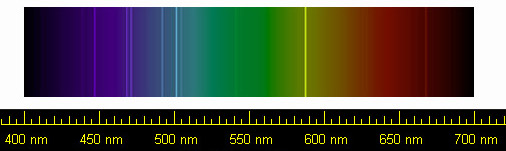
\includegraphics[width=12cm]{./resources/spectral_img/Helium_spectrum.jpg}
    \caption{Helium Spectral Image}
\end{figure}

\hypertarget{subsubsection::Li}{}\subsubsection{Lithium (Li)}

\textit{Number}: 3

\textit{Category}: AlkaliMetal

\textit{Phase at STP}: Solid

\textit{Appearance}: silvery-white

\textit{Density}: 0.534 g/L

\textit{Description}: Lithium is a chemical element with the symbol Li and atomic number 3. It is a soft, silver-white metal belonging to the alkali metal group of chemical elements. Under standard conditions it is the lightest metal and the least dense solid element.

\hypertarget{subsubsection::Be}{}\subsubsection{Beryllium (Be)}

\textit{Number}: 4

\textit{Category}: AlkalineEarthMetal

\textit{Phase at STP}: Solid

\textit{Appearance}: white-gray metallic

\textit{Density}: 1.85 g/L

\textit{Description}: Beryllium is a chemical element with symbol Be and atomic number 4. It is created through stellar nucleosynthesis and is a relatively rare element in the universe. It is a divalent element which occurs naturally only in combination with other elements in minerals.

\hypertarget{subsubsection::B}{}\subsubsection{Boron (B)}

\textit{Number}: 5

\textit{Category}: Metalloid

\textit{Phase at STP}: Solid

\textit{Appearance}: black-brown

\textit{Density}: 2.08 g/L

\textit{Description}: Boron is a metalloid chemical element with symbol B and atomic number 5. Produced entirely by cosmic ray spallation and supernovae and not by stellar nucleosynthesis, it is a low-abundance element in both the Solar system and the Earth's crust. Boron is concentrated on Earth by the water-solubility of its more common naturally occurring compounds, the borate minerals.

\hypertarget{subsubsection::C}{}\subsubsection{Carbon (C)}

\textit{Number}: 6

\textit{Category}: Nonmetal

\textit{Phase at STP}: Solid

\textit{Density}: 1.821 g/L

\textit{Description}: Carbon (from Latin:carbo) is a chemical element with symbol C and atomic number 6. On the periodic table, it is the first (row 2) of six elements in column (group) 14, which have in common the composition of their outer electron shell. It is nonmetallic and tetravalent-making four electrons available to form covalent chemical bonds.

\immediate\write18{sudo wget -nc -nd -q -r -P ./resources/spectral_img -A jpeg,jpg,bmp,gif,png https://upload.wikimedia.org/wikipedia/commons/8/8c/Carbon_Spectra.jpg}
\begin{figure}[!ht]
    \centering
    
\includegraphics[width=12cm]{./resources/spectral_img/Carbon_Spectra.jpg}
    \caption{Carbon Spectral Image}
\end{figure}

\hypertarget{subsubsection::N}{}\subsubsection{Nitrogen (N)}

\textit{Number}: 7

\textit{Category}: Nonmetal

\textit{Phase at STP}: Gas

\textit{Appearance}: colorless gas, liquid or solid

\textit{Density}: 1.251 g/L

\textit{Description}: Nitrogen is a chemical element with symbol N and atomic number 7. It is the lightest pnictogen and at room temperature, it is a transparent, odorless diatomic gas. Nitrogen is a common element in the universe, estimated at about seventh in total abundance in the Milky Way and the Solar System.

\immediate\write18{sudo wget -nc -nd -q -r -P ./resources/spectral_img -A jpeg,jpg,bmp,gif,png https://upload.wikimedia.org/wikipedia/commons/3/37/Nitrogen_Spectra.jpg}
\begin{figure}[!ht]
    \centering
    
\includegraphics[width=12cm]{./resources/spectral_img/Nitrogen_Spectra.jpg}
    \caption{Nitrogen Spectral Image}
\end{figure}

\hypertarget{subsubsection::O}{}\subsubsection{Oxygen (O)}

\textit{Number}: 8

\textit{Category}: Nonmetal

\textit{Phase at STP}: Gas

\textit{Density}: 1.429 g/L

\textit{Description}: Oxygen is a chemical element with symbol O and atomic number 8. It is a member of the chalcogen group on the periodic table and is a highly reactive nonmetal and oxidizing agent that readily forms compounds (notably oxides) with most elements. By mass, oxygen is the third-most abundant element in the universe, after hydrogen and helium.

\immediate\write18{sudo wget -nc -nd -q -r -P ./resources/spectral_img -A jpeg,jpg,bmp,gif,png https://upload.wikimedia.org/wikipedia/commons/a/a0/Oxygen_spectre.jpg}
\begin{figure}[!ht]
    \centering
    
\includegraphics[width=12cm]{./resources/spectral_img/Oxygen_spectre.jpg}
    \caption{Oxygen Spectral Image}
\end{figure}

\hypertarget{subsubsection::F}{}\subsubsection{Fluorine (F)}

\textit{Number}: 9

\textit{Category}: Nonmetal

\textit{Phase at STP}: Gas

\textit{Density}: 1.696 g/L

\textit{Description}: Fluorine is a chemical element with symbol F and atomic number 9. It is the lightest halogen and exists as a highly toxic pale yellow diatomic gas at standard conditions. As the most electronegative element, it is extremely reactive:almost all other elements, including some noble gases, form compounds with fluorine.

\hypertarget{subsubsection::Ne}{}\subsubsection{Neon (Ne)}

\textit{Number}: 10

\textit{Category}: NobleGas

\textit{Phase at STP}: Gas

\textit{Appearance}: colorless gas exhibiting an orange-red glow when placed in a high voltage electric field

\textit{Density}: 0.9002 g/L

\textit{Description}: Neon is a chemical element with symbol Ne and atomic number 10. It is in group 18 (noble gases) of the periodic table. Neon is a colorless, odorless, inert monatomic gas under standard conditions, with about two-thirds the density of air.

\immediate\write18{sudo wget -nc -nd -q -r -P ./resources/spectral_img -A jpeg,jpg,bmp,gif,png https://upload.wikimedia.org/wikipedia/commons/9/99/Neon_spectra.jpg}
\begin{figure}[!ht]
    \centering
    
\includegraphics[width=12cm]{./resources/spectral_img/Neon_spectra.jpg}
    \caption{Neon Spectral Image}
\end{figure}

\hypertarget{subsubsection::Na}{}\subsubsection{Sodium (Na)}

\textit{Number}: 11

\textit{Category}: AlkaliMetal

\textit{Phase at STP}: Solid

\textit{Appearance}: silvery white metallic

\textit{Density}: 0.968 g/L

\textit{Description}: Sodium is a chemical element with symbol Na and atomic number 11. It is a soft, silver-white, highly reactive metal. In the Periodic table it is in column 1 (alkali metals), and shares with the other six elements in that column that it has a single electron in its outer shell, which it readily donates, creating a positively charged atom - a cation.

\immediate\write18{sudo wget -nc -nd -q -r -P ./resources/spectral_img -A jpeg,jpg,bmp,gif,png https://upload.wikimedia.org/wikipedia/commons/0/0b/Sodium_Spectra.jpg}
\begin{figure}[!ht]
    \centering
    
\includegraphics[width=12cm]{./resources/spectral_img/Sodium_Spectra.jpg}
    \caption{Sodium Spectral Image}
\end{figure}

\hypertarget{subsubsection::Mg}{}\subsubsection{Magnesium (Mg)}

\textit{Number}: 12

\textit{Category}: AlkalineEarthMetal

\textit{Phase at STP}: Solid

\textit{Appearance}: shiny grey solid

\textit{Density}: 1.738 g/L

\textit{Description}: Magnesium is a chemical element with symbol Mg and atomic number 12. It is a shiny gray solid which bears a close physical resemblance to the other five elements in the second column (Group 2, or alkaline earth metals) of the periodic table:they each have the same electron configuration in their outer electron shell producing a similar crystal structure. Magnesium is the ninth most abundant element in the universe.

\immediate\write18{sudo wget -nc -nd -q -r -P ./resources/spectral_img -A jpeg,jpg,bmp,gif,png https://upload.wikimedia.org/wikipedia/commons/a/a0/Magnesium_Spectra.jpg}
\begin{figure}[!ht]
    \centering
    
\includegraphics[width=12cm]{./resources/spectral_img/Magnesium_Spectra.jpg}
    \caption{Magnesium Spectral Image}
\end{figure}

\hypertarget{subsubsection::Al}{}\subsubsection{Aluminium (Al)}

\textit{Number}: 13

\textit{Category}: PostTransitionMetal

\textit{Phase at STP}: Solid

\textit{Appearance}: silvery gray metallic

\textit{Density}: 2.7 g/L

\textit{Description}: Aluminium (or aluminum; see different endings) is a chemical element in the boron group with symbol Al and atomic number 13. It is a silvery-white, soft, nonmagnetic, ductile metal. Aluminium is the third most abundant element (after oxygen and silicon), and the most abundant metal, in the Earth's crust.

\hypertarget{subsubsection::Si}{}\subsubsection{Silicon (Si)}

\textit{Number}: 14

\textit{Category}: Metalloid

\textit{Phase at STP}: Solid

\textit{Appearance}: crystalline, reflective with bluish-tinged faces

\textit{Density}: 2.329 g/L

\textit{Description}: Silicon is a chemical element with symbol Si and atomic number 14. It is a tetravalent metalloid, more reactive than germanium, the metalloid directly below it in the table. Controversy about silicon's character dates to its discovery.

\immediate\write18{sudo wget -nc -nd -q -r -P ./resources/spectral_img -A jpeg,jpg,bmp,gif,png https://upload.wikimedia.org/wikipedia/commons/0/0b/Silicon_Spectra.jpg}
\begin{figure}[!ht]
    \centering
    
\includegraphics[width=12cm]{./resources/spectral_img/Silicon_Spectra.jpg}
    \caption{Silicon Spectral Image}
\end{figure}

\hypertarget{subsubsection::P}{}\subsubsection{Phosphorus (P)}

\textit{Number}: 15

\textit{Category}: Nonmetal

\textit{Phase at STP}: Solid

\textit{Appearance}: colourless, waxy white, yellow, scarlet, red, violet, black

\textit{Density}: 1.823 g/L

\textit{Description}: Phosphorus is a chemical element with symbol P and atomic number 15. As an element, phosphorus exists in two major forms-white phosphorus and red phosphorus - but due to its high reactivity, phosphorus is never found as a free element on Earth. Instead phosphorus-containing minerals are almost always present in their maximally oxidised state, as inorganic phosphate rocks.

\hypertarget{subsubsection::S}{}\subsubsection{Sulfur (S)}

\textit{Number}: 16

\textit{Category}: Nonmetal

\textit{Phase at STP}: Solid

\textit{Appearance}: lemon yellow sintered microcrystals

\textit{Density}: 2.07 g/L

\textit{Description}: Sulfur or sulphur (see spelling differences) is a chemical element with symbol S and atomic number 16. It is an abundant, multivalent non-metal. Under normal conditions, sulfur atoms form cyclic octatomic molecules with chemical formula S8.

\immediate\write18{sudo wget -nc -nd -q -r -P ./resources/spectral_img -A jpeg,jpg,bmp,gif,png https://upload.wikimedia.org/wikipedia/commons/b/b4/Sulfur_Spectrum.jpg}
\begin{figure}[!ht]
    \centering
    
\includegraphics[width=12cm]{./resources/spectral_img/Sulfur_Spectrum.jpg}
    \caption{Sulfur Spectral Image}
\end{figure}

\hypertarget{subsubsection::Cl}{}\subsubsection{Chlorine (Cl)}

\textit{Number}: 17

\textit{Category}: Nonmetal

\textit{Phase at STP}: Gas

\textit{Appearance}: pale yellow-green gas

\textit{Density}: 3.2 g/L

\textit{Description}: Chlorine is a chemical element with symbol Cl and atomic number 17. It also has a relative atomic mass of 35.5. Chlorine is in the halogen group (17) and is the second lightest halogen following fluorine.

\immediate\write18{sudo wget -nc -nd -q -r -P ./resources/spectral_img -A jpeg,jpg,bmp,gif,png https://upload.wikimedia.org/wikipedia/commons/6/61/Chlorine_spectrum_visible.png}
\begin{figure}[!ht]
    \centering
    
\includegraphics[width=12cm]{./resources/spectral_img/Chlorine_spectrum_visible.png}
    \caption{Chlorine Spectral Image}
\end{figure}

\hypertarget{subsubsection::Ar}{}\subsubsection{Argon (Ar)}

\textit{Number}: 18

\textit{Category}: NobleGas

\textit{Phase at STP}: Gas

\textit{Appearance}: colorless gas exhibiting a lilac/violet glow when placed in a high voltage electric field

\textit{Density}: 1.784 g/L

\textit{Description}: Argon is a chemical element with symbol Ar and atomic number 18. It is in group 18 of the periodic table and is a noble gas. Argon is the third most common gas in the Earth's atmosphere, at 0.934% (9,340 ppmv), making it over twice as abundant as the next most common atmospheric gas, water vapor (which averages about 4000 ppmv, but varies greatly), and 23 times as abundant as the next most common non-condensing atmospheric gas, carbon dioxide (400 ppmv), and more than 500 times as abundant as the next most common noble gas, neon (18 ppmv).

\immediate\write18{sudo wget -nc -nd -q -r -P ./resources/spectral_img -A jpeg,jpg,bmp,gif,png https://upload.wikimedia.org/wikipedia/commons/3/37/Argon_Spectrum.png}
\begin{figure}[!ht]
    \centering
    
\includegraphics[width=12cm]{./resources/spectral_img/Argon_Spectrum.png}
    \caption{Argon Spectral Image}
\end{figure}

\hypertarget{subsubsection::K}{}\subsubsection{Potassium (K)}

\textit{Number}: 19

\textit{Category}: AlkaliMetal

\textit{Phase at STP}: Solid

\textit{Appearance}: silvery gray

\textit{Density}: 0.862 g/L

\textit{Description}: Potassium is a chemical element with symbol K (derived from Neo-Latin, kalium) and atomic number 19. It was first isolated from potash, the ashes of plants, from which its name is derived. In the Periodic table, potassium is one of seven elements in column (group) 1 (alkali metals):they all have a single valence electron in their outer electron shell, which they readily give up to create an atom with a positive charge - a cation, and combine with anions to form salts.

\immediate\write18{sudo wget -nc -nd -q -r -P ./resources/spectral_img -A jpeg,jpg,bmp,gif,png https://upload.wikimedia.org/wikipedia/commons/d/d0/Potassium_Spectrum.jpg}
\begin{figure}[!ht]
    \centering
    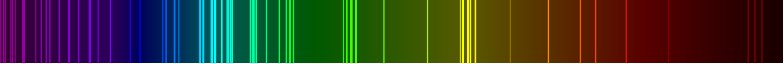
\includegraphics[width=12cm]{./resources/spectral_img/Potassium_Spectrum.jpg}
    \caption{Potassium Spectral Image}
\end{figure}

\hypertarget{subsubsection::Ca}{}\subsubsection{Calcium (Ca)}

\textit{Number}: 20

\textit{Category}: AlkalineEarthMetal

\textit{Phase at STP}: Solid

\textit{Density}: 1.55 g/L

\textit{Description}: Calcium is a chemical element with symbol Ca and atomic number 20. Calcium is a soft gray alkaline earth metal, fifth-most-abundant element by mass in the Earth's crust. The ion Ca2+ is also the fifth-most-abundant dissolved ion in seawater by both molarity and mass, after sodium, chloride, magnesium, and sulfate.

\immediate\write18{sudo wget -nc -nd -q -r -P ./resources/spectral_img -A jpeg,jpg,bmp,gif,png https://upload.wikimedia.org/wikipedia/commons/2/21/Calcium_Spectrum.png}
\begin{figure}[!ht]
    \centering
    
\includegraphics[width=12cm]{./resources/spectral_img/Calcium_Spectrum.png}
    \caption{Calcium Spectral Image}
\end{figure}

\hypertarget{subsubsection::Sc}{}\subsubsection{Scandium (Sc)}

\textit{Number}: 21

\textit{Category}: TransitionMetal

\textit{Phase at STP}: Solid

\textit{Appearance}: silvery white

\textit{Density}: 2.985 g/L

\textit{Description}: Scandium is a chemical element with symbol Sc and atomic number 21. A silvery-white metallic d-block element, it has historically been sometimes classified as a rare earth element, together with yttrium and the lanthanoids. It was discovered in 1879 by spectral analysis of the minerals euxenite and gadolinite from Scandinavia.

\hypertarget{subsubsection::Ti}{}\subsubsection{Titanium (Ti)}

\textit{Number}: 22

\textit{Category}: TransitionMetal

\textit{Phase at STP}: Solid

\textit{Appearance}: silvery grey-white metallic

\textit{Density}: 4.506 g/L

\textit{Description}: Titanium is a chemical element with symbol Ti and atomic number 22. It is a lustrous transition metal with a silver color, low density and high strength. It is highly resistant to corrosion in sea water, aqua regia and chlorine.

\hypertarget{subsubsection::V}{}\subsubsection{Vanadium (V)}

\textit{Number}: 23

\textit{Category}: TransitionMetal

\textit{Phase at STP}: Solid

\textit{Appearance}: blue-silver-grey metal

\textit{Density}: 6.0 g/L

\textit{Description}: Vanadium is a chemical element with symbol V and atomic number 23. It is a hard, silvery grey, ductile and malleable transition metal. The element is found only in chemically combined form in nature, but once isolated artificially, the formation of an oxide layer stabilizes the free metal somewhat against further oxidation.

\hypertarget{subsubsection::Cr}{}\subsubsection{Chromium (Cr)}

\textit{Number}: 24

\textit{Category}: TransitionMetal

\textit{Phase at STP}: Solid

\textit{Appearance}: silvery metallic

\textit{Density}: 7.19 g/L

\textit{Description}: Chromium is a chemical element with symbol Cr and atomic number 24. It is the first element in Group 6. It is a steely-gray, lustrous, hard and brittle metal which takes a high polish, resists tarnishing, and has a high melting point.

\hypertarget{subsubsection::Mn}{}\subsubsection{Manganese (Mn)}

\textit{Number}: 25

\textit{Category}: TransitionMetal

\textit{Phase at STP}: Solid

\textit{Appearance}: silvery metallic

\textit{Density}: 7.21 g/L

\textit{Description}: Manganese is a chemical element with symbol Mn and atomic number 25. It is not found as a free element in nature; it is often found in combination with iron, and in many minerals. Manganese is a metal with important industrial metal alloy uses, particularly in stainless steels.

\hypertarget{subsubsection::Fe}{}\subsubsection{Iron (Fe)}

\textit{Number}: 26

\textit{Category}: TransitionMetal

\textit{Phase at STP}: Solid

\textit{Appearance}: lustrous metallic with a grayish tinge

\textit{Density}: 7.874 g/L

\textit{Description}: Iron is a chemical element with symbol Fe (from Latin:ferrum) and atomic number 26. It is a metal in the first transition series. It is by mass the most common element on Earth, forming much of Earth's outer and inner core.

\immediate\write18{sudo wget -nc -nd -q -r -P ./resources/spectral_img -A jpeg,jpg,bmp,gif,png https://upload.wikimedia.org/wikipedia/commons/6/6a/Iron_Spectrum.jpg}
\begin{figure}[!ht]
    \centering
    
\includegraphics[width=12cm]{./resources/spectral_img/Iron_Spectrum.jpg}
    \caption{Iron Spectral Image}
\end{figure}

\hypertarget{subsubsection::Co}{}\subsubsection{Cobalt (Co)}

\textit{Number}: 27

\textit{Category}: TransitionMetal

\textit{Phase at STP}: Solid

\textit{Appearance}: hard lustrous gray metal

\textit{Density}: 8.9 g/L

\textit{Description}: Cobalt is a chemical element with symbol Co and atomic number 27. Like nickel, cobalt in the Earth's crust is found only in chemically combined form, save for small deposits found in alloys of natural meteoric iron. The free element, produced by reductive smelting, is a hard, lustrous, silver-gray metal.

\hypertarget{subsubsection::Ni}{}\subsubsection{Nickel (Ni)}

\textit{Number}: 28

\textit{Category}: TransitionMetal

\textit{Phase at STP}: Solid

\textit{Appearance}: lustrous, metallic, and silver with a gold tinge

\textit{Density}: 8.908 g/L

\textit{Description}: Nickel is a chemical element with symbol Ni and atomic number 28. It is a silvery-white lustrous metal with a slight golden tinge. Nickel belongs to the transition metals and is hard and ductile.

\hypertarget{subsubsection::Cu}{}\subsubsection{Copper (Cu)}

\textit{Number}: 29

\textit{Category}: TransitionMetal

\textit{Phase at STP}: Solid

\textit{Appearance}: red-orange metallic luster

\textit{Density}: 8.96 g/L

\textit{Description}: Copper is a chemical element with symbol Cu (from Latin:cuprum) and atomic number 29. It is a soft, malleable and ductile metal with very high thermal and electrical conductivity. A freshly exposed surface of pure copper has a reddish-orange color.

\hypertarget{subsubsection::Zn}{}\subsubsection{Zinc (Zn)}

\textit{Number}: 30

\textit{Category}: TransitionMetal

\textit{Phase at STP}: Solid

\textit{Appearance}: silver-gray

\textit{Density}: 7.14 g/L

\textit{Description}: Zinc, in commerce also spelter, is a chemical element with symbol Zn and atomic number 30. It is the first element of group 12 of the periodic table. In some respects zinc is chemically similar to magnesium:its ion is of similar size and its only common oxidation state is +2.

\hypertarget{subsubsection::Ga}{}\subsubsection{Gallium (Ga)}

\textit{Number}: 31

\textit{Category}: PostTransitionMetal

\textit{Phase at STP}: Solid

\textit{Appearance}: silver-white

\textit{Density}: 5.91 g/L

\textit{Description}: Gallium is a chemical element with symbol Ga and atomic number 31. Elemental gallium does not occur in free form in nature, but as the gallium(III) compounds that are in trace amounts in zinc ores and in bauxite. Gallium is a soft, silvery metal, and elemental gallium is a brittle solid at low temperatures, and melts at 29.76 ºC (85.57 ºF) (slightly above room temperature).

\hypertarget{subsubsection::Ge}{}\subsubsection{Germanium (Ge)}

\textit{Number}: 32

\textit{Category}: Metalloid

\textit{Phase at STP}: Solid

\textit{Appearance}: grayish-white

\textit{Density}: 5.323 g/L

\textit{Description}: Germanium is a chemical element with symbol Ge and atomic number 32. It is a lustrous, hard, grayish-white metalloid in the carbon group, chemically similar to its group neighbors tin and silicon. Purified germanium is a semiconductor, with an appearance most similar to elemental silicon.

\hypertarget{subsubsection::As}{}\subsubsection{Arsenic (As)}

\textit{Number}: 33

\textit{Category}: Metalloid

\textit{Phase at STP}: Solid

\textit{Appearance}: metallic grey

\textit{Density}: 5.727 g/L

\textit{Description}: Arsenic is a chemical element with symbol As and atomic number 33. Arsenic occurs in many minerals, usually in conjunction with sulfur and metals, and also as a pure elemental crystal. Arsenic is a metalloid.

\hypertarget{subsubsection::Se}{}\subsubsection{Selenium (Se)}

\textit{Number}: 34

\textit{Category}: Nonmetal

\textit{Phase at STP}: Solid

\textit{Appearance}: black, red, and gray (not pictured) allotropes

\textit{Density}: 4.81 g/L

\textit{Description}: Selenium is a chemical element with symbol Se and atomic number 34. It is a nonmetal with properties that are intermediate between those of its periodic table column-adjacent chalcogen elements sulfur and tellurium. It rarely occurs in its elemental state in nature, or as pure ore compounds.

\hypertarget{subsubsection::Br}{}\subsubsection{Bromine (Br)}

\textit{Number}: 35

\textit{Category}: Nonmetal

\textit{Phase at STP}: Liquid

\textit{Density}: 23.1028 g/L

\textit{Description}: Bromine is a chemical element with symbol Br, and atomic number 35. It is a halogen. The element was isolated independently by two chemists, Carl Jacob Lowig and Antoine Jerome Balard, in 1825.

\hypertarget{subsubsection::Kr}{}\subsubsection{Krypton (Kr)}

\textit{Number}: 36

\textit{Category}: NobleGas

\textit{Phase at STP}: Gas

\textit{Appearance}: colorless gas, exhibiting a whitish glow in a high electric field

\textit{Density}: 3.749 g/L

\textit{Description}: Krypton (from Greek: kryptos the hidden one) is a chemical element with symbol Kr and atomic number 36. It is a member of group 18 (noble gases) elements. A colorless, odorless, tasteless noble gas, krypton occurs in trace amounts in the atmosphere, is isolated by fractionally distilling liquefied air, and is often used with other rare gases in fluorescent lamps.

\immediate\write18{sudo wget -nc -nd -q -r -P ./resources/spectral_img -A jpeg,jpg,bmp,gif,png https://upload.wikimedia.org/wikipedia/commons/a/a6/Krypton_Spectrum.jpg}
\begin{figure}[!ht]
    \centering
    
\includegraphics[width=12cm]{./resources/spectral_img/Krypton_Spectrum.jpg}
    \caption{Krypton Spectral Image}
\end{figure}

\hypertarget{subsubsection::Rb}{}\subsubsection{Rubidium (Rb)}

\textit{Number}: 37

\textit{Category}: AlkaliMetal

\textit{Phase at STP}: Solid

\textit{Appearance}: grey white

\textit{Density}: 1.532 g/L

\textit{Description}: Rubidium is a chemical element with symbol Rb and atomic number 37. Rubidium is a soft, silvery-white metallic element of the alkali metal group, with an atomic mass of 85.4678. Elemental rubidium is highly reactive, with properties similar to those of other alkali metals, such as very rapid oxidation in air.

\hypertarget{subsubsection::Sr}{}\subsubsection{Strontium (Sr)}

\textit{Number}: 38

\textit{Category}: AlkalineEarthMetal

\textit{Phase at STP}: Solid

\textit{Density}: 2.64 g/L

\textit{Description}: Strontium is a chemical element with symbol Sr and atomic number 38. An alkaline earth metal, strontium is a soft silver-white or yellowish metallic element that is highly reactive chemically. The metal turns yellow when it is exposed to air.

\hypertarget{subsubsection::Y}{}\subsubsection{Yttrium (Y)}

\textit{Number}: 39

\textit{Category}: TransitionMetal

\textit{Phase at STP}: Solid

\textit{Appearance}: silvery white

\textit{Density}: 4.472 g/L

\textit{Description}: Yttrium is a chemical element with symbol Y and atomic number 39. It is a silvery-metallic transition metal chemically similar to the lanthanides and it has often been classified as a rare earth element. Yttrium is almost always found combined with the lanthanides in rare earth minerals and is never found in nature as a free element.

\hypertarget{subsubsection::Zr}{}\subsubsection{Zirconium (Zr)}

\textit{Number}: 40

\textit{Category}: TransitionMetal

\textit{Phase at STP}: Solid

\textit{Appearance}: silvery white

\textit{Density}: 6.52 g/L

\textit{Description}: Zirconium is a chemical element with symbol Zr and atomic number 40. The name of zirconium is taken from the name of the mineral zircon, the most important source of zirconium. The word zircon comes from the Persian word zargun, meaning gold-colored.

\hypertarget{subsubsection::Nb}{}\subsubsection{Niobium (Nb)}

\textit{Number}: 41

\textit{Category}: TransitionMetal

\textit{Phase at STP}: Solid

\textit{Appearance}: gray metallic, bluish when oxidized

\textit{Density}: 8.57 g/L

\textit{Description}: Niobium, formerly columbium, is a chemical element with symbol Nb (formerly Cb) and atomic number 41. It is a soft, grey, ductile transition metal, which is often found in the pyrochlore mineral, the main commercial source for niobium, and columbite. The name comes from Greek mythology: Niobe, daughter of Tantalus since it is so similar to tantalum.

\hypertarget{subsubsection::Mo}{}\subsubsection{Molybdenum (Mo)}

\textit{Number}: 42

\textit{Category}: TransitionMetal

\textit{Phase at STP}: Solid

\textit{Appearance}: gray metallic

\textit{Density}: 10.28 g/L

\textit{Description}: Molybdenum is a chemical element with symbol Mo and atomic number 42. The name is from Neo-Latin molybdaenum, from Ancient Greek molybdos, meaning lead, since its ores were confused with lead ores. Molybdenum minerals have been known throughout history, but the element was discovered (in the sense of differentiating it as a new entity from the mineral salts of other metals) in 1778 by Carl Wilhelm Scheele.

\hypertarget{subsubsection::Tc}{}\subsubsection{Technetium (Tc)}

\textit{Number}: 43

\textit{Category}: TransitionMetal

\textit{Phase at STP}: Solid

\textit{Appearance}: shiny gray metal

\textit{Density}: 11 g/L

\textit{Description}: Technetium is a chemical element with symbol Tc and atomic number 43. It is the element with the lowest atomic number in the periodic table that has no stable isotopes:every form of it is radioactive. Nearly all technetium is produced synthetically, and only minute amounts are found in nature.

\hypertarget{subsubsection::Ru}{}\subsubsection{Ruthenium (Ru)}

\textit{Number}: 44

\textit{Category}: TransitionMetal

\textit{Phase at STP}: Solid

\textit{Appearance}: silvery white metallic

\textit{Density}: 12.45 g/L

\textit{Description}: Ruthenium is a chemical element with symbol Ru and atomic number 44. It is a rare transition metal belonging to the platinum group of the periodic table. Like the other metals of the platinum group, ruthenium is inert to most other chemicals.

\hypertarget{subsubsection::Rh}{}\subsubsection{Rhodium (Rh)}

\textit{Number}: 45

\textit{Category}: TransitionMetal

\textit{Phase at STP}: Solid

\textit{Appearance}: silvery white metallic

\textit{Density}: 12.41 g/L

\textit{Description}: Rhodium is a chemical element with symbol Rh and atomic number 45. It is a rare, silvery-white, hard, and chemically inert transition metal. It is a member of the platinum group.

\hypertarget{subsubsection::Pd}{}\subsubsection{Palladium (Pd)}

\textit{Number}: 46

\textit{Category}: TransitionMetal

\textit{Phase at STP}: Solid

\textit{Appearance}: silvery white

\textit{Density}: 12.023 g/L

\textit{Description}: Palladium is a chemical element with symbol Pd and atomic number 46. It is a rare and lustrous silvery-white metal discovered in 1803 by William Hyde Wollaston. He named it after the asteroid Pallas, which was itself named after the epithet of the Greek goddess Athena, acquired by her when she slew Pallas.

\hypertarget{subsubsection::Ag}{}\subsubsection{Silver (Ag)}

\textit{Number}: 47

\textit{Category}: TransitionMetal

\textit{Phase at STP}: Solid

\textit{Appearance}: lustrous white metal

\textit{Density}: 10.49 g/L

\textit{Description}: Silver is a chemical element with symbol Ag (Latin:argentum, from the Indo-European root for grey or shining) and atomic number 47. A soft, white, lustrous transition metal, it possesses the highest electrical conductivity, thermal conductivity and reflectivity of any metal. The metal occurs naturally in its pure, free form (native silver), as an alloy with gold and other metals, and in minerals such as argentite and chlorargyrite.

\hypertarget{subsubsection::Cd}{}\subsubsection{Cadmium (Cd)}

\textit{Number}: 48

\textit{Category}: TransitionMetal

\textit{Phase at STP}: Solid

\textit{Appearance}: silvery bluish-gray metallic

\textit{Density}: 8.65 g/L

\textit{Description}: Cadmium is a chemical element with symbol Cd and atomic number 48. This soft, bluish-white metal is chemically similar to the two other stable metals in group 12, zinc and mercury. Like zinc, it prefers oxidation state +2 in most of its compounds and like mercury it shows a low melting point compared to transition metals.

\hypertarget{subsubsection::In}{}\subsubsection{Indium (In)}

\textit{Number}: 49

\textit{Category}: PostTransitionMetal

\textit{Phase at STP}: Solid

\textit{Appearance}: silvery lustrous gray

\textit{Density}: 7.31 g/L

\textit{Description}: Indium is a chemical element with symbol In and atomic number 49. It is a post-transition metallic element that is rare in Earth's crust. The metal is very soft, malleable and easily fusible, with a melting point higher than sodium, but lower than lithium or tin.

\hypertarget{subsubsection::Sn}{}\subsubsection{Tin (Sn)}

\textit{Number}: 50

\textit{Category}: PostTransitionMetal

\textit{Phase at STP}: Solid

\textit{Appearance}: silvery-white (beta) or gray (alpha)

\textit{Density}: 7.365 g/L

\textit{Description}: Tin is a chemical element with the symbol Sn (for Latin:stannum) and atomic number 50. It is a main group metal in group 14 of the periodic table. Tin shows a chemical similarity to both neighboring group-14 elements, germanium and lead, and has two possible oxidation states, +2 and the slightly more stable +4.

\hypertarget{subsubsection::Sb}{}\subsubsection{Antimony (Sb)}

\textit{Number}: 51

\textit{Category}: Metalloid

\textit{Phase at STP}: Solid

\textit{Appearance}: silvery lustrous gray

\textit{Density}: 6.697 g/L

\textit{Description}: Antimony is a chemical element with symbol Sb (from Latin:stibium) and atomic number 51. A lustrous gray metalloid, it is found in nature mainly as the sulfide mineral stibnite (Sb2S3). Antimony compounds have been known since ancient times and were used for cosmetics; metallic antimony was also known, but it was erroneously identified as lead upon its discovery.

\hypertarget{subsubsection::Te}{}\subsubsection{Tellurium (Te)}

\textit{Number}: 52

\textit{Category}: Metalloid

\textit{Phase at STP}: Solid

\textit{Density}: 6.24 g/L

\textit{Description}: Tellurium is a chemical element with symbol Te and atomic number 52. It is a brittle, mildly toxic, rare, silver-white metalloid. Tellurium is chemically related to selenium and sulfur.

\hypertarget{subsubsection::I}{}\subsubsection{Iodine (I)}

\textit{Number}: 53

\textit{Category}: Nonmetal

\textit{Phase at STP}: Solid

\textit{Appearance}: lustrous metallic gray, violet as a gas

\textit{Density}: 4.933 g/L

\textit{Description}: Iodine is a chemical element with symbol I and atomic number 53. The name is from Greek, meaning violet or purple, due to the color of iodine vapor. Iodine and its compounds are primarily used in nutrition, and industrially in the production of acetic acid and certain polymers.

\hypertarget{subsubsection::Xe}{}\subsubsection{Xenon (Xe)}

\textit{Number}: 54

\textit{Category}: NobleGas

\textit{Phase at STP}: Gas

\textit{Appearance}: colorless gas, exhibiting a blue glow when placed in a high voltage electric field

\textit{Density}: 5.894 g/L

\textit{Description}: Xenon is a chemical element with symbol Xe and atomic number 54. It is a colorless, dense, odorless noble gas, that occurs in the Earth's atmosphere in trace amounts. Although generally unreactive, xenon can undergo a few chemical reactions such as the formation of xenon hexafluoroplatinate, the first noble gas compound to be synthesized.

\immediate\write18{sudo wget -nc -nd -q -r -P ./resources/spectral_img -A jpeg,jpg,bmp,gif,png https://upload.wikimedia.org/wikipedia/commons/6/67/Xenon_Spectrum.jpg}
\begin{figure}[!ht]
    \centering
    
\includegraphics[width=12cm]{./resources/spectral_img/Xenon_Spectrum.jpg}
    \caption{Xenon Spectral Image}
\end{figure}

\hypertarget{subsubsection::Cs}{}\subsubsection{Cesium (Cs)}

\textit{Number}: 55

\textit{Category}: AlkaliMetal

\textit{Phase at STP}: Solid

\textit{Appearance}: silvery gold

\textit{Density}: 1.93 g/L

\textit{Description}: Caesium or cesium is a chemical element with symbol Cs and atomic number 55. It is a soft, silvery-gold alkali metal with a melting point of 28 ºC (82 ºF), which makes it one of only five elemental metals that are liquid at or near room temperature. Caesium is an alkali metal and has physical and chemical properties similar to those of rubidium and potassium.

\hypertarget{subsubsection::Ba}{}\subsubsection{Barium (Ba)}

\textit{Number}: 56

\textit{Category}: AlkalineEarthMetal

\textit{Phase at STP}: Solid

\textit{Density}: 3.51 g/L

\textit{Description}: Barium is a chemical element with symbol Ba and atomic number 56. It is the fifth element in Group 2, a soft silvery metallic alkaline earth metal. Because of its high chemical reactivity barium is never found in nature as a free element.

\hypertarget{subsubsection::La}{}\subsubsection{Lanthanum (La)}

\textit{Number}: 57

\textit{Category}: Lanthanide

\textit{Phase at STP}: Solid

\textit{Appearance}: silvery white

\textit{Density}: 6.162 g/L

\textit{Description}: Lanthanum is a soft, ductile, silvery-white metallic chemical element with symbol La and atomic number 57. It tarnishes rapidly when exposed to air and is soft enough to be cut with a knife. It gave its name to the lanthanide series, a group of 15 similar elements between lanthanum and lutetium in the periodic table:it is also sometimes considered the first element of the 6th-period transition metals.

\hypertarget{subsubsection::Ce}{}\subsubsection{Cerium (Ce)}

\textit{Number}: 58

\textit{Category}: Lanthanide

\textit{Phase at STP}: Solid

\textit{Appearance}: silvery white

\textit{Density}: 6.77 g/L

\textit{Description}: Cerium is a chemical element with symbol Ce and atomic number 58. It is a soft, silvery, ductile metal which easily oxidizes in air. Cerium was named after the dwarf planet Ceres (itself named after the Roman goddess of agriculture).

\hypertarget{subsubsection::Pr}{}\subsubsection{Praseodymium (Pr)}

\textit{Number}: 59

\textit{Category}: Lanthanide

\textit{Phase at STP}: Solid

\textit{Appearance}: grayish white

\textit{Density}: 6.77 g/L

\textit{Description}: Praseodymium is a chemical element with symbol Pr and atomic number 59. Praseodymium is a soft, silvery, malleable and ductile metal in the lanthanide group. It is valued for its magnetic, electrical, chemical, and optical properties.

\hypertarget{subsubsection::Nd}{}\subsubsection{Neodymium (Nd)}

\textit{Number}: 60

\textit{Category}: Lanthanide

\textit{Phase at STP}: Solid

\textit{Appearance}: silvery white

\textit{Density}: 7.01 g/L

\textit{Description}: Neodymium is a chemical element with symbol Nd and atomic number 60. It is a soft silvery metal that tarnishes in air. Neodymium was discovered in 1885 by the Austrian chemist Carl Auer von Welsbach.

\hypertarget{subsubsection::Pm}{}\subsubsection{Promethium (Pm)}

\textit{Number}: 61

\textit{Category}: Lanthanide

\textit{Phase at STP}: Solid

\textit{Appearance}: metallic

\textit{Density}: 7.26 g/L

\textit{Description}: Promethium, originally prometheum, is a chemical element with the symbol Pm and atomic number 61. All of its isotopes are radioactive; it is one of only two such elements that are followed in the periodic table by elements with stable forms, a distinction shared with technetium. Chemically, promethium is a lanthanide, which forms salts when combined with other elements.

\hypertarget{subsubsection::Sm}{}\subsubsection{Samarium (Sm)}

\textit{Number}: 62

\textit{Category}: Lanthanide

\textit{Phase at STP}: Solid

\textit{Appearance}: silvery white

\textit{Density}: 7.52 g/L

\textit{Description}: Samarium is a chemical element with symbol Sm and atomic number 62. It is a moderately hard silvery metal that readily oxidizes in air. Being a typical member of the lanthanide series, samarium usually assumes the oxidation state +3.

\hypertarget{subsubsection::Eu}{}\subsubsection{Europium (Eu)}

\textit{Number}: 63

\textit{Category}: Lanthanide

\textit{Phase at STP}: Solid

\textit{Density}: 5.264 g/L

\textit{Description}: Europium is a chemical element with symbol Eu and atomic number 63. It was isolated in 1901 and is named after the continent of Europe. It is a moderately hard, silvery metal which readily oxidizes in air and water.

\hypertarget{subsubsection::Gd}{}\subsubsection{Gadolinium (Gd)}

\textit{Number}: 64

\textit{Category}: Lanthanide

\textit{Phase at STP}: Solid

\textit{Appearance}: silvery white

\textit{Density}: 7.9 g/L

\textit{Description}: Gadolinium is a chemical element with symbol Gd and atomic number 64. It is a silvery-white, malleable and ductile rare-earth metal. It is found in nature only in combined (salt) form.

\hypertarget{subsubsection::Tb}{}\subsubsection{Terbium (Tb)}

\textit{Number}: 65

\textit{Category}: Lanthanide

\textit{Phase at STP}: Solid

\textit{Appearance}: silvery white

\textit{Density}: 8.23 g/L

\textit{Description}: Terbium is a chemical element with symbol Tb and atomic number 65. It is a silvery-white rare earth metal that is malleable, ductile and soft enough to be cut with a knife. Terbium is never found in nature as a free element, but it is contained in many minerals, including cerite, gadolinite, monazite, xenotime and euxenite.

\hypertarget{subsubsection::Dy}{}\subsubsection{Dysprosium (Dy)}

\textit{Number}: 66

\textit{Category}: Lanthanide

\textit{Phase at STP}: Solid

\textit{Appearance}: silvery white

\textit{Density}: 8.54 g/L

\textit{Description}: Dysprosium is a chemical element with the symbol Dy and atomic number 66. It is a rare earth element with a metallic silver luster. Dysprosium is never found in nature as a free element, though it is found in various minerals, such as xenotime.

\hypertarget{subsubsection::Ho}{}\subsubsection{Holmium (Ho)}

\textit{Number}: 67

\textit{Category}: Lanthanide

\textit{Phase at STP}: Solid

\textit{Appearance}: silvery white

\textit{Density}: 8.79 g/L

\textit{Description}: Holmium is a chemical element with symbol Ho and atomic number 67. Part of the lanthanide series, holmium is a rare earth element. Holmium was discovered by Swedish chemist Per Theodor Cleve.

\hypertarget{subsubsection::Er}{}\subsubsection{Erbium (Er)}

\textit{Number}: 68

\textit{Category}: Lanthanide

\textit{Phase at STP}: Solid

\textit{Appearance}: silvery white

\textit{Density}: 9.066 g/L

\textit{Description}: Erbium is a chemical element in the lanthanide series, with symbol Er and atomic number 68. A silvery-white solid metal when artificially isolated, natural erbium is always found in chemical combination with other elements on Earth. As such, it is a rare earth element which is associated with several other rare elements in the mineral gadolinite from Ytterby in Sweden, where yttrium, ytterbium, and terbium were discovered.

\hypertarget{subsubsection::Tm}{}\subsubsection{Thulium (Tm)}

\textit{Number}: 69

\textit{Category}: Lanthanide

\textit{Phase at STP}: Solid

\textit{Appearance}: silvery gray

\textit{Density}: 9.32 g/L

\textit{Description}: Thulium is a chemical element with symbol Tm and atomic number 69. It is the thirteenth and antepenultimate (third-last) element in the lanthanide series. Like the other lanthanides, the most common oxidation state is +3, seen in its oxide, halides and other compounds.

\hypertarget{subsubsection::Yb}{}\subsubsection{Ytterbium (Yb)}

\textit{Number}: 70

\textit{Category}: Lanthanide

\textit{Phase at STP}: Solid

\textit{Density}: 6.9 g/L

\textit{Description}: Ytterbium is a chemical element with symbol Yb and atomic number 70. It is the fourteenth and penultimate element in the lanthanide series, which is the basis of the relative stability of its +2 oxidation state. However, like the other lanthanides, its most common oxidation state is +3, seen in its oxide, halides and other compounds.

\hypertarget{subsubsection::Lu}{}\subsubsection{Lutetium (Lu)}

\textit{Number}: 71

\textit{Category}: Lanthanide

\textit{Phase at STP}: Solid

\textit{Appearance}: silvery white

\textit{Density}: 9.841 g/L

\textit{Description}: Lutetium is a chemical element with symbol Lu and atomic number 71. It is a silvery white metal, which resists corrosion in dry, but not in moist air. It is considered the first element of the 6th-period transition metals and the last element in the lanthanide series, and is traditionally counted among the rare earths.

\hypertarget{subsubsection::Hf}{}\subsubsection{Hafnium (Hf)}

\textit{Number}: 72

\textit{Category}: TransitionMetal

\textit{Phase at STP}: Solid

\textit{Appearance}: steel gray

\textit{Density}: 13.31 g/L

\textit{Description}: Hafnium is a chemical element with symbol Hf and atomic number 72. A lustrous, silvery gray, tetravalent transition metal, hafnium chemically resembles zirconium and is found in zirconium minerals. Its existence was predicted by Dmitri Mendeleev in 1869, though it was not identified until 1923, making it the penultimate stable element to be discovered (rhenium was identified two years later).

\immediate\write18{sudo wget -nc -nd -q -r -P ./resources/spectral_img -A jpeg,jpg,bmp,gif,png https://upload.wikimedia.org/wikipedia/commons/a/ac/Hafnium_spectrum_visible.png}
\begin{figure}[!ht]
    \centering
    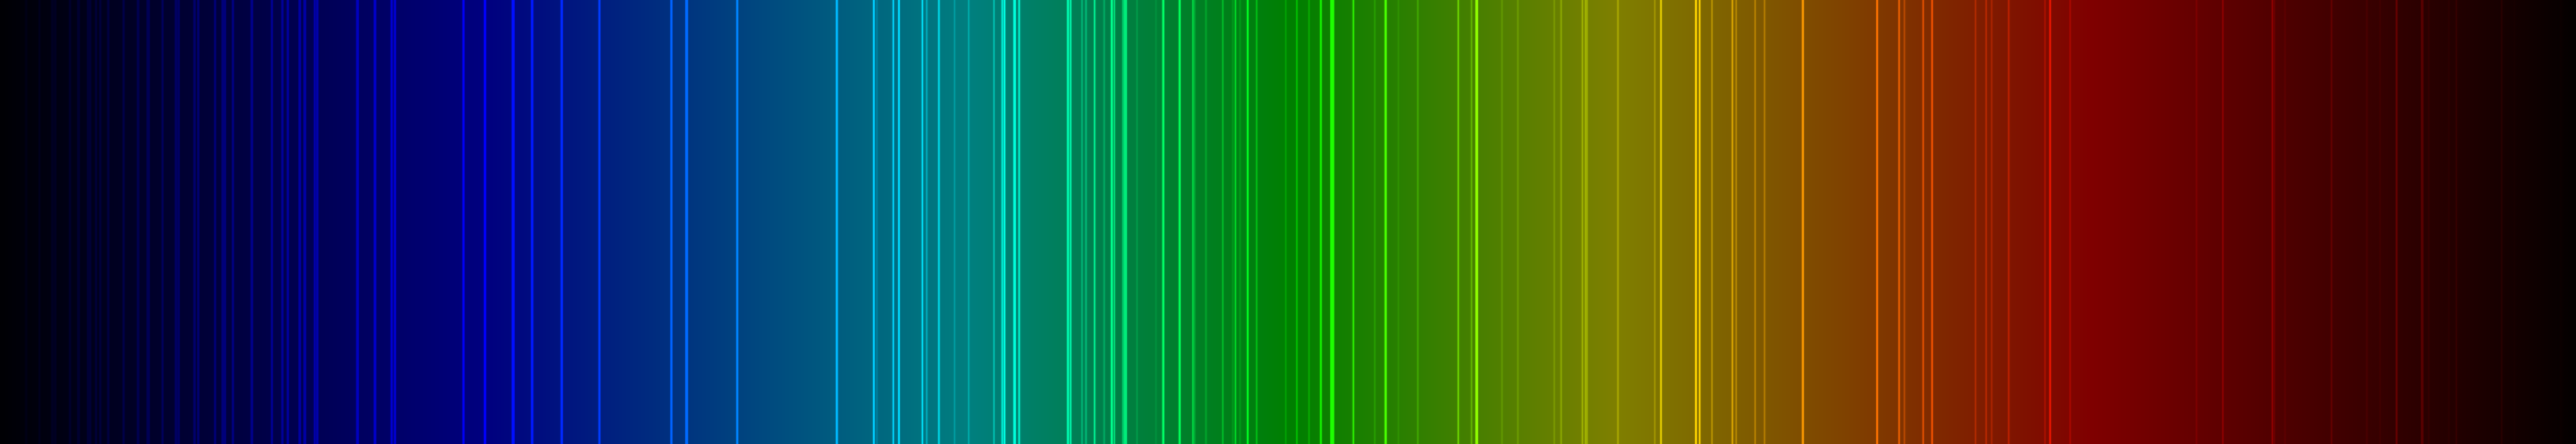
\includegraphics[width=12cm]{./resources/spectral_img/Hafnium_spectrum_visible.png}
    \caption{Hafnium Spectral Image}
\end{figure}

\hypertarget{subsubsection::Ta}{}\subsubsection{Tantalum (Ta)}

\textit{Number}: 73

\textit{Category}: TransitionMetal

\textit{Phase at STP}: Solid

\textit{Appearance}: gray blue

\textit{Density}: 16.69 g/L

\textit{Description}: Tantalum is a chemical element with symbol Ta and atomic number 73. Previously known as tantalium, its name comes from Tantalus, an antihero from Greek mythology. Tantalum is a rare, hard, blue-gray, lustrous transition metal that is highly corrosion-resistant.

\immediate\write18{sudo wget -nc -nd -q -r -P ./resources/spectral_img -A jpeg,jpg,bmp,gif,png https://upload.wikimedia.org/wikipedia/commons/a/a6/Tantalum_spectrum_visible.png}
\begin{figure}[!ht]
    \centering
    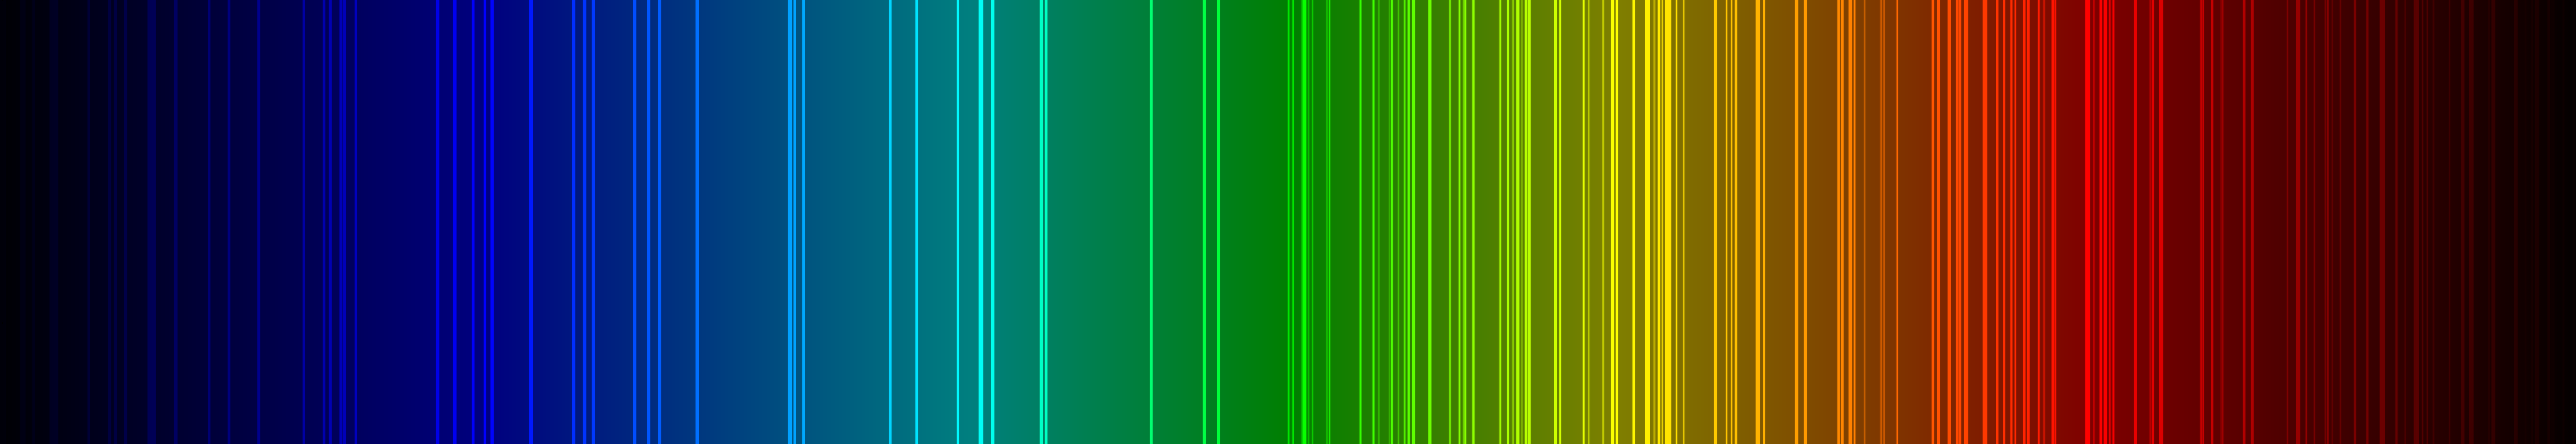
\includegraphics[width=12cm]{./resources/spectral_img/Tantalum_spectrum_visible.png}
    \caption{Tantalum Spectral Image}
\end{figure}

\hypertarget{subsubsection::W}{}\subsubsection{Tungsten (W)}

\textit{Number}: 74

\textit{Category}: TransitionMetal

\textit{Phase at STP}: Solid

\textit{Appearance}: grayish white, lustrous

\textit{Density}: 19.25 g/L

\textit{Description}: Tungsten, also known as wolfram, is a chemical element with symbol W and atomic number 74. The word tungsten comes from the Swedish language tung sten, which directly translates to heavy stone. Its name in Swedish is volfram, however, in order to distinguish it from scheelite, which in Swedish is alternatively named tungsten.

\hypertarget{subsubsection::Re}{}\subsubsection{Rhenium (Re)}

\textit{Number}: 75

\textit{Category}: TransitionMetal

\textit{Phase at STP}: Solid

\textit{Appearance}: silvery-grayish

\textit{Density}: 21.02 g/L

\textit{Description}: Rhenium is a chemical element with symbol Re and atomic number 75. It is a silvery-white, heavy, third-row transition metal in group 7 of the periodic table. With an estimated average concentration of 1 part per billion (ppb), rhenium is one of the rarest elements in the Earth's crust.

\hypertarget{subsubsection::Os}{}\subsubsection{Osmium (Os)}

\textit{Number}: 76

\textit{Category}: TransitionMetal

\textit{Phase at STP}: Solid

\textit{Appearance}: silvery, blue cast

\textit{Density}: 22.59 g/L

\textit{Description}: Osmium (from Greek osme meaning smell) is a chemical element with symbol Os and atomic number 76. It is a hard, brittle, bluish-white transition metal in the platinum group that is found as a trace element in alloys, mostly in platinum ores. Osmium is the densest naturally occurring element, with a density of 22.59 g/cm3.

\hypertarget{subsubsection::Ir}{}\subsubsection{Iridium (Ir)}

\textit{Number}: 77

\textit{Category}: TransitionMetal

\textit{Phase at STP}: Solid

\textit{Appearance}: silvery white

\textit{Density}: 22.56 g/L

\textit{Description}: Iridium is a chemical element with symbol Ir and atomic number 77. A very hard, brittle, silvery-white transition metal of the platinum group, iridium is generally credited with being the second densest element (after osmium) based on measured density, although calculations involving the space lattices of the elements show that iridium is denser. It is also the most corrosion-resistant metal, even at temperatures as high as 2000 ºC. Although only certain molten salts and halogens are corrosive to solid iridium, finely divided iridium dust is much more reactive and can be flammable.

\hypertarget{subsubsection::Pt}{}\subsubsection{Platinum (Pt)}

\textit{Number}: 78

\textit{Category}: TransitionMetal

\textit{Phase at STP}: Solid

\textit{Appearance}: silvery white

\textit{Density}: 21.45 g/L

\textit{Description}: Platinum is a chemical element with symbol Pt and atomic number 78. It is a dense, malleable, ductile, highly unreactive, precious, gray-white transition metal. Its name is derived from the Spanish term platina, which is literally translated into little silver.

\hypertarget{subsubsection::Au}{}\subsubsection{Gold (Au)}

\textit{Number}: 79

\textit{Category}: TransitionMetal

\textit{Phase at STP}: Solid

\textit{Appearance}: metallic yellow

\textit{Density}: 19.3 g/L

\textit{Description}: Gold is a chemical element with symbol Au (from Latin:aurum) and atomic number 79. In its purest form, it is a bright, slightly reddish yellow, dense, soft, malleable and ductile metal. Chemically, gold is a transition metal and a group 11 element.

\hypertarget{subsubsection::Hg}{}\subsubsection{Mercury (Hg)}

\textit{Number}: 80

\textit{Category}: TransitionMetal

\textit{Phase at STP}: Liquid

\textit{Appearance}: silvery

\textit{Density}: 13.534 g/L

\textit{Description}: Mercury is a chemical element with symbol Hg and atomic number 80. It is commonly known as quicksilver and was formerly named hydrargyrum. A heavy, silvery d-block element, mercury is the only metallic element that is liquid at standard conditions for temperature and pressure; the only other element that is liquid under these conditions is bromine, though metals such as caesium, gallium, and rubidium melt just above room temperature.

\hypertarget{subsubsection::Tl}{}\subsubsection{Thallium (Tl)}

\textit{Number}: 81

\textit{Category}: PostTransitionMetal

\textit{Phase at STP}: Solid

\textit{Appearance}: silvery white

\textit{Density}: 11.85 g/L

\textit{Description}: Thallium is a chemical element with symbol Tl and atomic number 81. This soft gray post-transition metal is not found free in nature. When isolated, it resembles tin, but discolors when exposed to air.

\hypertarget{subsubsection::Pb}{}\subsubsection{Lead (Pb)}

\textit{Number}: 82

\textit{Category}: PostTransitionMetal

\textit{Phase at STP}: Solid

\textit{Appearance}: metallic gray

\textit{Density}: 11.34 g/L

\textit{Description}: Lead is a chemical element in the carbon group with symbol Pb (from Latin:plumbum) and atomic number 82. Lead is a soft, malleable and heavy post-transition metal. Metallic lead has a bluish-white color after being freshly cut, but it soon tarnishes to a dull grayish color when exposed to air.

\hypertarget{subsubsection::Bi}{}\subsubsection{Bismuth (Bi)}

\textit{Number}: 83

\textit{Category}: PostTransitionMetal

\textit{Phase at STP}: Solid

\textit{Appearance}: lustrous silver

\textit{Density}: 9.78 g/L

\textit{Description}: Bismuth is a chemical element with symbol Bi and atomic number 83. Bismuth, a pentavalent post-transition metal, chemically resembles arsenic and antimony. Elemental bismuth may occur naturally, although its sulfide and oxide form important commercial ores.

\hypertarget{subsubsection::Po}{}\subsubsection{Polonium (Po)}

\textit{Number}: 84

\textit{Category}: PostTransitionMetal

\textit{Phase at STP}: Solid

\textit{Appearance}: silvery

\textit{Density}: 9.196 g/L

\textit{Description}: Polonium is a chemical element with symbol Po and atomic number 84, discovered in 1898 by Marie Curie and Pierre Curie. A rare and highly radioactive element with no stable isotopes, polonium is chemically similar to bismuth and tellurium, and it occurs in uranium ores. Applications of polonium are few.

\hypertarget{subsubsection::At}{}\subsubsection{Astatine (At)}

\textit{Number}: 85

\textit{Category}: Metalloid

\textit{Phase at STP}: Solid

\textit{Appearance}: unknown, probably metallic

\textit{Density}: 26.35 g/L

\textit{Description}: Astatine is a very rare radioactive chemical element with the chemical symbol At and atomic number 85. It occurs on Earth as the decay product of various heavier elements. All its isotopes are short-lived; the most stable is astatine-210, with a half-life of 8.1 hours.

\hypertarget{subsubsection::Rn}{}\subsubsection{Radon (Rn)}

\textit{Number}: 86

\textit{Category}: NobleGas

\textit{Phase at STP}: Gas

\textit{Appearance}: colorless gas, occasionally glows green or red in discharge tubes

\textit{Density}: 9.73 g/L

\textit{Description}: Radon is a chemical element with symbol Rn and atomic number 86. It is a radioactive, colorless, odorless, tasteless noble gas, occurring naturally as a decay product of radium. Its most stable isotope, 222Rn, has a half-life of 3.8 days.

\immediate\write18{sudo wget -nc -nd -q -r -P ./resources/spectral_img -A jpeg,jpg,bmp,gif,png https://upload.wikimedia.org/wikipedia/commons/0/0d/Radon_spectrum.png}
\begin{figure}[!ht]
    \centering
    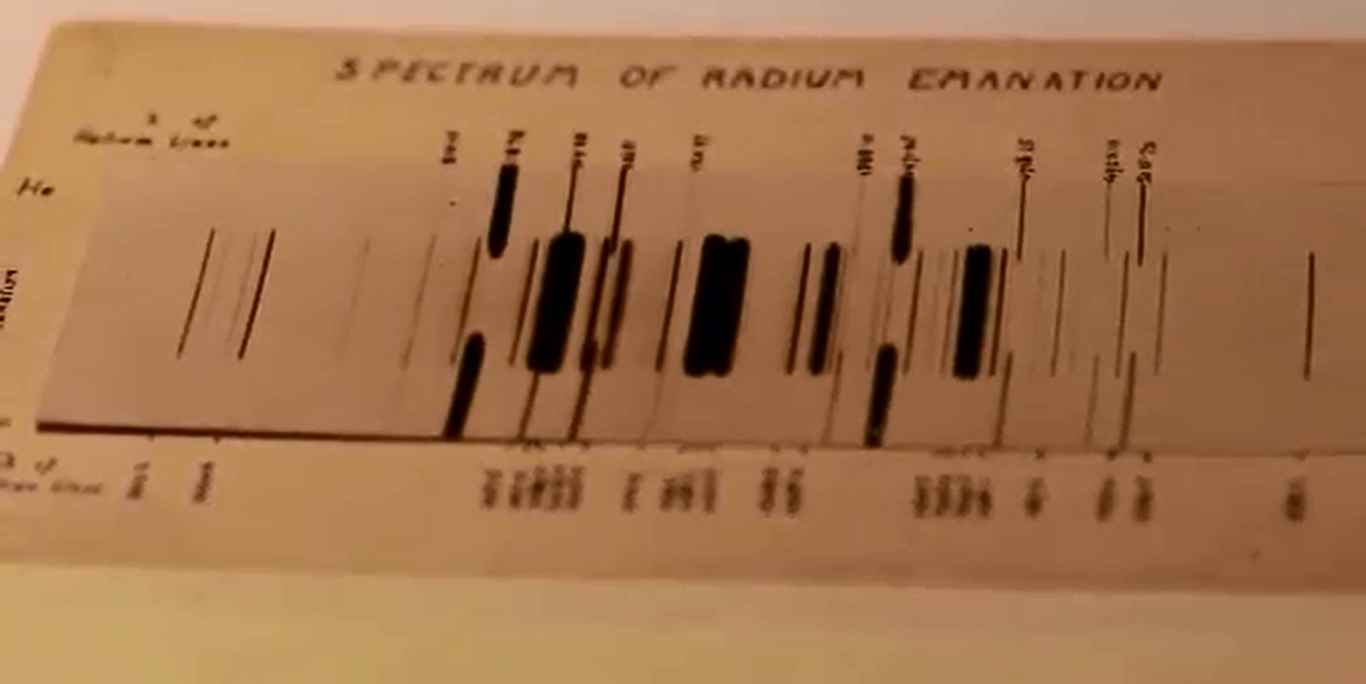
\includegraphics[width=12cm]{./resources/spectral_img/Radon_spectrum.png}
    \caption{Radon Spectral Image}
\end{figure}

\hypertarget{subsubsection::Fr}{}\subsubsection{Francium (Fr)}

\textit{Number}: 87

\textit{Category}: AlkaliMetal

\textit{Phase at STP}: Solid

\textit{Density}: 1.87 g/L

\textit{Description}: Francium is a chemical element with symbol Fr and atomic number 87. It used to be known as eka-caesium and actinium K. It is the second-least electronegative element, behind only caesium. Francium is a highly radioactive metal that decays into astatine, radium, and radon.

\hypertarget{subsubsection::Ra}{}\subsubsection{Radium (Ra)}

\textit{Number}: 88

\textit{Category}: AlkalineEarthMetal

\textit{Phase at STP}: Solid

\textit{Appearance}: silvery white metallic

\textit{Density}: 5.5 g/L

\textit{Description}: Radium is a chemical element with symbol Ra and atomic number 88. It is the sixth element in group 2 of the periodic table, also known as the alkaline earth metals. Pure radium is almost colorless, but it readily combines with nitrogen (rather than oxygen) on exposure to air, forming a black surface layer of radium nitride (Ra3N2).

\hypertarget{subsubsection::Ac}{}\subsubsection{Actinium (Ac)}

\textit{Number}: 89

\textit{Category}: Actinide

\textit{Phase at STP}: Solid

\textit{Density}: 10 g/L

\textit{Description}: Actinium is a radioactive chemical element with symbol Ac (not to be confused with the abbreviation for an acetyl group) and atomic number 89, which was discovered in 1899. It was the first non-primordial radioactive element to be isolated. Polonium, radium and radon were observed before actinium, but they were not isolated until 1902.

\hypertarget{subsubsection::Th}{}\subsubsection{Thorium (Th)}

\textit{Number}: 90

\textit{Category}: Actinide

\textit{Phase at STP}: Solid

\textit{Appearance}: silvery, often with black tarnish

\textit{Density}: 11.724 g/L

\textit{Description}: Thorium is a chemical element with symbol Th and atomic number 90. A radioactive actinide metal, thorium is one of only two significantly radioactive elements that still occur naturally in large quantities as a primordial element (the other being uranium). It was discovered in 1828 by the Norwegian Reverend and amateur mineralogist Morten Thrane Esmark and identified by the Swedish chemist Jons Jakob Berzelius, who named it after Thor, the Norse god of thunder.

\hypertarget{subsubsection::Pa}{}\subsubsection{Protactinium (Pa)}

\textit{Number}: 91

\textit{Category}: Actinide

\textit{Phase at STP}: Solid

\textit{Appearance}: bright, silvery metallic luster

\textit{Density}: 15.37 g/L

\textit{Description}: Protactinium is a chemical element with symbol Pa and atomic number 91. It is a dense, silvery-gray metal which readily reacts with oxygen, water vapor and inorganic acids. It forms various chemical compounds where protactinium is usually present in the oxidation state +5, but can also assume +4 and even +2 or +3 states.

\hypertarget{subsubsection::U}{}\subsubsection{Uranium (U)}

\textit{Number}: 92

\textit{Category}: Actinide

\textit{Phase at STP}: Solid

\textit{Density}: 19.1 g/L

\textit{Description}: Uranium is a chemical element with symbol U and atomic number 92. It is a silvery-white metal in the actinide series of the periodic table. A uranium atom has 92 protons and 92 electrons, of which 6 are valence electrons.

\hypertarget{subsubsection::Np}{}\subsubsection{Neptunium (Np)}

\textit{Number}: 93

\textit{Category}: Actinide

\textit{Phase at STP}: Solid

\textit{Appearance}: silvery metallic

\textit{Density}: 20.45 g/L

\textit{Description}: Neptunium is a chemical element with symbol Np and atomic number 93. A radioactive actinide metal, neptunium is the first transuranic element. Its position in the periodic table just after uranium, named after the planet Uranus, led to it being named after Neptune, the next planet beyond Uranus.

\hypertarget{subsubsection::Pu}{}\subsubsection{Plutonium (Pu)}

\textit{Number}: 94

\textit{Category}: Actinide

\textit{Phase at STP}: Solid

\textit{Appearance}: silvery white, tarnishing to dark gray in air

\textit{Density}: 19.816 g/L

\textit{Description}: Plutonium is a transuranic radioactive chemical element with symbol Pu and atomic number 94. It is an actinide metal of silvery-gray appearance that tarnishes when exposed to air, and forms a dull coating when oxidized. The element normally exhibits six allotropes and four oxidation states.

\hypertarget{subsubsection::Am}{}\subsubsection{Americium (Am)}

\textit{Number}: 95

\textit{Category}: Actinide

\textit{Phase at STP}: Solid

\textit{Appearance}: silvery white

\textit{Density}: 12 g/L

\textit{Description}: Americium is a radioactive transuranic chemical element with symbol Am and atomic number 95. This member of the actinide series is located in the periodic table under the lanthanide element europium, and thus by analogy was named after the Americas. Americium was first produced in 1944 by the group of Glenn T.Seaborg from Berkeley, California, at the metallurgical laboratory of University of Chicago.

\immediate\write18{sudo wget -nc -nd -q -r -P ./resources/spectral_img -A jpeg,jpg,bmp,gif,png https://upload.wikimedia.org/wikipedia/commons/3/37/Americium_spectrum_visible.png}
\begin{figure}[!ht]
    \centering
    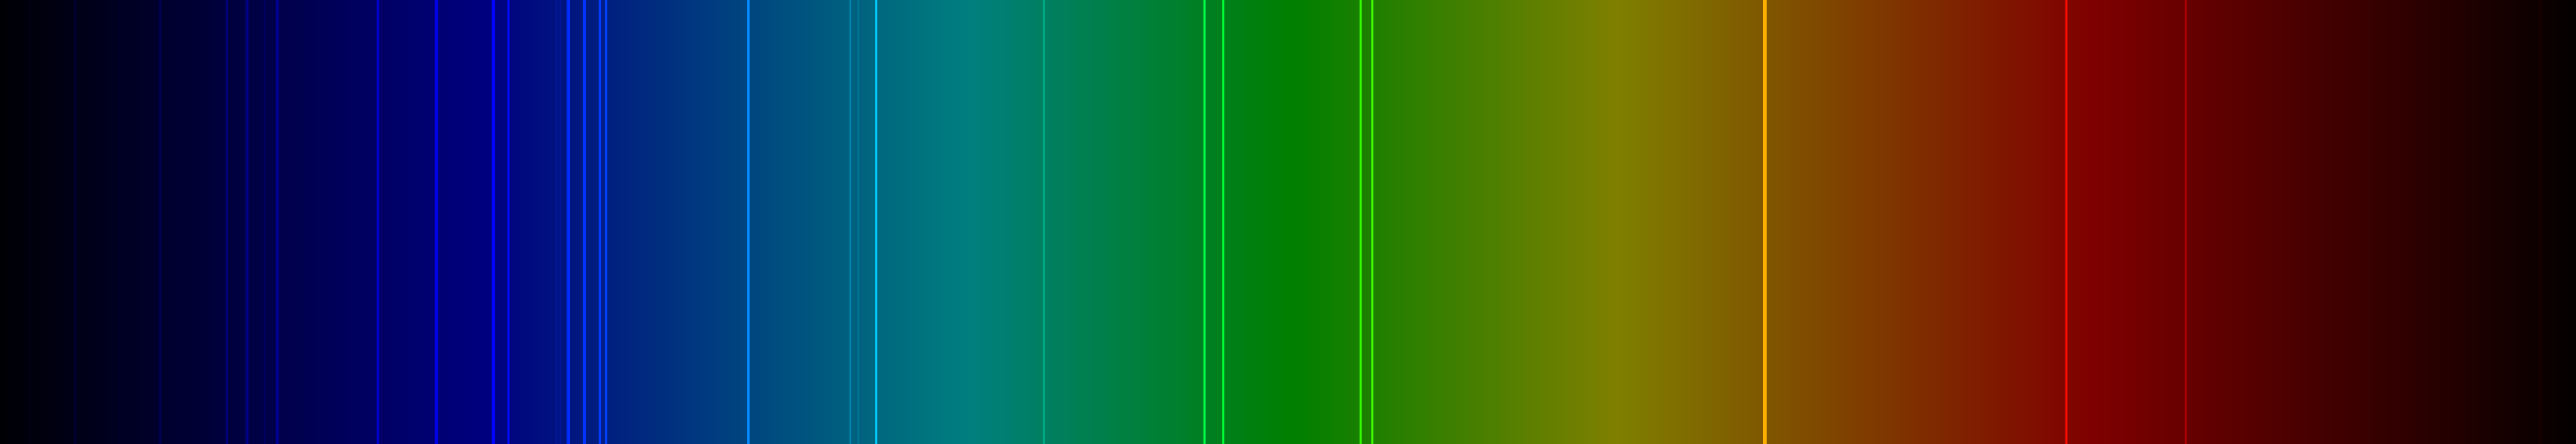
\includegraphics[width=12cm]{./resources/spectral_img/Americium_spectrum_visible.png}
    \caption{Americium Spectral Image}
\end{figure}

\hypertarget{subsubsection::Cm}{}\subsubsection{Curium (Cm)}

\textit{Number}: 96

\textit{Category}: Actinide

\textit{Phase at STP}: Solid

\textit{Appearance}: silvery metallic, glows purple in the dark

\textit{Density}: 13.51 g/L

\textit{Description}: Curium is a transuranic radioactive chemical element with symbol Cm and atomic number 96. This element of the actinide series was named after Marie and Pierre Curie - both were known for their research on radioactivity. Curium was first intentionally produced and identified in July 1944 by the group of Glenn T. Seaborg at the University of California, Berkeley.

\hypertarget{subsubsection::Bk}{}\subsubsection{Berkelium (Bk)}

\textit{Number}: 97

\textit{Category}: Actinide

\textit{Phase at STP}: Solid

\textit{Appearance}: silvery

\textit{Density}: 14.78 g/L

\textit{Description}: Berkelium is a transuranic radioactive chemical element with symbol Bk and atomic number 97. It is a member of the actinide and transuranium element series. It is named after the city of Berkeley, California, the location of the University of California Radiation Laboratory where it was discovered in December 1949.

\hypertarget{subsubsection::Cf}{}\subsubsection{Californium (Cf)}

\textit{Number}: 98

\textit{Category}: Actinide

\textit{Phase at STP}: Solid

\textit{Appearance}: silvery

\textit{Density}: 15.1 g/L

\textit{Description}: Californium is a radioactive metallic chemical element with symbol Cf and atomic number 98. The element was first made in 1950 at the University of California Radiation Laboratory in Berkeley, by bombarding curium with alpha particles (helium-4 ions). It is an actinide element, the sixth transuranium element to be synthesized, and has the second-highest atomic mass of all the elements that have been produced in amounts large enough to see with the unaided eye (after einsteinium).

\hypertarget{subsubsection::Es}{}\subsubsection{Einsteinium (Es)}

\textit{Number}: 99

\textit{Category}: Actinide

\textit{Phase at STP}: Solid

\textit{Appearance}: silver-colored

\textit{Density}: 8.84 g/L

\textit{Description}: Einsteinium is a synthetic element with symbol Es and atomic number 99. It is the seventh transuranic element, and an actinide. Einsteinium was discovered as a component of the debris of the first hydrogen bomb explosion in 1952, and named after Albert Einstein.

\hypertarget{subsubsection::Fm}{}\subsubsection{Fermium (Fm)}

\textit{Number}: 100

\textit{Category}: Actinide

\textit{Phase at STP}: Solid

\textit{Description}: Fermium is a synthetic element with symbol Fm and atomic number 100. It is a member of the actinide series. It is the heaviest element that can be formed by neutron bombardment of lighter elements, and hence the last element that can be prepared in macroscopic quantities, although pure fermium metal has not yet been prepared.

\hypertarget{subsubsection::Md}{}\subsubsection{Mendelevium (Md)}

\textit{Number}: 101

\textit{Category}: Actinide

\textit{Phase at STP}: Solid

\textit{Description}: Mendelevium is a synthetic element with chemical symbol Md (formerly Mv) and atomic number 101. A metallic radioactive transuranic element in the actinide series, it is the first element that currently cannot be produced in macroscopic quantities through neutron bombardment of lighter elements. It is the antepenultimate actinide and the ninth transuranic element.

\hypertarget{subsubsection::No}{}\subsubsection{Nobelium (No)}

\textit{Number}: 102

\textit{Category}: Actinide

\textit{Phase at STP}: Solid

\textit{Description}: Nobelium is a synthetic chemical element with symbol No and atomic number 102. It is named in honor of Alfred Nobel, the inventor of dynamite and benefactor of science. A radioactive metal, it is the tenth transuranic element and is the penultimate member of the actinide series.

\hypertarget{subsubsection::Lr}{}\subsubsection{Lawrencium (Lr)}

\textit{Number}: 103

\textit{Category}: Actinide

\textit{Phase at STP}: Solid

\textit{Description}: Lawrencium is a synthetic chemical element with chemical symbol Lr (formerly Lw) and atomic number 103. It is named in honor of Ernest Lawrence, inventor of the cyclotron, a device that was used to discover many artificial radioactive elements. A radioactive metal, lawrencium is the eleventh transuranic element and is also the final member of the actinide series.

\hypertarget{subsubsection::Rf}{}\subsubsection{Rutherfordium (Rf)}

\textit{Number}: 104

\textit{Category}: TransitionMetal

\textit{Phase at STP}: Solid

\textit{Density}: 23.2 g/L

\textit{Description}: Rutherfordium is a chemical element with symbol Rf and atomic number 104, named in honor of physicist Ernest Rutherford. It is a synthetic element (an element that can be created in a laboratory but is not found in nature) and radioactive; the most stable known isotope, 267Rf, has a half-life of approximately 1.3 hours. In the periodic table of the elements, it is a d - block element and the second of the fourth - row transition elements.

\hypertarget{subsubsection::Db}{}\subsubsection{Dubnium (Db)}

\textit{Number}: 105

\textit{Category}: TransitionMetal

\textit{Phase at STP}: Solid

\textit{Density}: 29.3 g/L

\textit{Description}: Dubnium is a chemical element with symbol Db and atomic number 105. It is named after the town of Dubna in Russia (north of Moscow), where it was first produced. It is a synthetic element (an element that can be created in a laboratory but is not found in nature) and radioactive; the most stable known isotope, dubnium-268, has a half-life of approximately 28 hours.

\hypertarget{subsubsection::Sg}{}\subsubsection{Seaborgium (Sg)}

\textit{Number}: 106

\textit{Category}: TransitionMetal

\textit{Phase at STP}: Solid

\textit{Density}: 35.0 g/L

\textit{Description}: Seaborgium is a synthetic element with symbol Sg and atomic number 106. Its most stable isotope 271Sg has a half-life of 1.9 minutes. A more recently discovered isotope 269Sg has a potentially slightly longer half-life (ca.

\hypertarget{subsubsection::Bh}{}\subsubsection{Bohrium (Bh)}

\textit{Number}: 107

\textit{Category}: TransitionMetal

\textit{Phase at STP}: Solid

\textit{Density}: 37.1 g/L

\textit{Description}: Bohrium is a chemical element with symbol Bh and atomic number 107. It is named after Danish physicist Niels Bohr. It is a synthetic element (an element that can be created in a laboratory but is not found in nature) and radioactive; the most stable known isotope, 270Bh, has a half-life of approximately 61 seconds.

\hypertarget{subsubsection::Hs}{}\subsubsection{Hassium (Hs)}

\textit{Number}: 108

\textit{Category}: TransitionMetal

\textit{Phase at STP}: Solid

\textit{Density}: 40.7 g/L

\textit{Description}: Hassium is a chemical element with symbol Hs and atomic number 108, named after the German state of Hesse. It is a synthetic element (an element that can be created in a laboratory but is not found in nature) and radioactive; the most stable known isotope, 269Hs, has a half-life of approximately 9.7 seconds, although an unconfirmed metastable state, 277mHs, may have a longer half-life of about 130 seconds. More than 100 atoms of hassium have been synthesized to date.

\hypertarget{subsubsection::Mt}{}\subsubsection{Meitnerium (Mt)}

\textit{Number}: 109

\textit{Category}: Unknown

\textit{Phase at STP}: Solid

\textit{Density}: 37.4 g/L

\textit{Description}: Meitnerium is a chemical element with symbol Mt and atomic number 109. It is an extremely radioactive synthetic element (an element not found in nature that can be created in a laboratory). The most stable known isotope, meitnerium-278, has a half-life of 7.6 seconds.

\hypertarget{subsubsection::Ds}{}\subsubsection{Darmstadtium (Ds)}

\textit{Number}: 110

\textit{Category}: Unknown

\textit{Phase at STP}: Solid

\textit{Density}: 34.8 g/L

\textit{Description}: Darmstadtium is a chemical element with symbol Ds and atomic number 110. It is an extremely radioactive synthetic element. The most stable known isotope, darmstadtium-281, has a half-life of approximately 10 seconds.

\hypertarget{subsubsection::Rg}{}\subsubsection{Roentgenium (Rg)}

\textit{Number}: 111

\textit{Category}: Unknown

\textit{Phase at STP}: Solid

\textit{Density}: 28.7 g/L

\textit{Description}: Roentgenium is a chemical element with symbol Rg and atomic number 111. It is an extremely radioactive synthetic element (an element that can be created in a laboratory but is not found in nature); the most stable known isotope, roentgenium-282, has a half-life of 2.1 minutes. Roentgenium was first created in 1994 by the GSI Helmholtz Centre for Heavy Ion Research near Darmstadt, Germany.

\hypertarget{subsubsection::Cn}{}\subsubsection{Copernicium (Cn)}

\textit{Number}: 112

\textit{Category}: TransitionMetal

\textit{Phase at STP}: Gas

\textit{Density}: 23.7 g/L

\textit{Description}: Copernicium is a chemical element with symbol Cn and atomic number 112. It is an extremely radioactive synthetic element that can only be created in a laboratory. The most stable known isotope, copernicium-285, has a half-life of approximately 29 seconds, but it is possible that this copernicium isotope may have a nuclear isomer with a longer half-life, 8.9 min.

\hypertarget{subsubsection::Nh}{}\subsubsection{Nihonium (Nh)}

\textit{Number}: 113

\textit{Category}: Unknown

\textit{Phase at STP}: Solid

\textit{Density}: 16 g/L

\textit{Description}: Nihonium is a chemical element with atomic number 113. It has a symbol Nh. It is a synthetic element (an element that can be created in a laboratory but is not found in nature) and is extremely radioactive; its most stable known isotope, nihonium-286, has a half-life of 20 seconds.

\hypertarget{subsubsection::Fl}{}\subsubsection{Flerovium (Fl)}

\textit{Number}: 114

\textit{Category}: PostTransitionMetal

\textit{Phase at STP}: Solid

\textit{Density}: 14 g/L

\textit{Description}: Flerovium is a superheavy artificial chemical element with symbol Fl and atomic number 114. It is an extremely radioactive synthetic element. The element is named after the Flerov Laboratory of Nuclear Reactions of the Joint Institute for Nuclear Research in Dubna, Russia, where the element was discovered in 1998.

\hypertarget{subsubsection::Mc}{}\subsubsection{Moscovium (Mc)}

\textit{Number}: 115

\textit{Category}: Unknown

\textit{Phase at STP}: Solid

\textit{Density}: 13.5 g/L

\textit{Description}: Moscovium is the name of a synthetic superheavy element in the periodic table that has the symbol Mc and has the atomic number 115. It is an extremely radioactive element; its most stable known isotope, moscovium-289, has a half-life of only 220 milliseconds. It is also known as eka-bismuth or simply element 115.

\hypertarget{subsubsection::Lv}{}\subsubsection{Livermorium (Lv)}

\textit{Number}: 116

\textit{Category}: Unknown

\textit{Phase at STP}: Solid

\textit{Density}: 12.9 g/L

\textit{Description}: Livermorium is a synthetic superheavy element with symbol Lv and atomic number 116. It is an extremely radioactive element that has only been created in the laboratory and has not been observed in nature. The element is named after the Lawrence Livermore National Laboratory in the United States, which collaborated with the Joint Institute for Nuclear Research in Dubna, Russia to discover livermorium in 2000.

\hypertarget{subsubsection::Ts}{}\subsubsection{Tennessine (Ts)}

\textit{Number}: 117

\textit{Category}: Unknown

\textit{Phase at STP}: Solid

\textit{Density}: 7.17 g/L

\textit{Description}: Tennessine is a superheavy artificial chemical element with an atomic number of 117 and a symbol of Ts. Also known as eka-astatine or element 117, it is the second-heaviest known element and penultimate element of the 7th period of the periodic table. As of 2016, fifteen tennessine atoms have been observed:six when it was first synthesized in 2010, seven in 2012, and two in 2014.

\hypertarget{subsubsection::Og}{}\subsubsection{Oganesson (Og)}

\textit{Number}: 118

\textit{Category}: Unknown

\textit{Phase at STP}: Solid

\textit{Density}: 4.95 g/L

\textit{Description}: Oganesson is IUPAC's name for the transactinide element with the atomic number 118 and element symbol Og. It is also known as eka-radon or element 118, and on the periodic table of the elements it is a p-block element and the last one of the 7th period. Oganesson is currently the only synthetic member of group 18.

\end{document}
